\documentclass{beamer}
%
% Choose how your presentation looks.
%
% For more themes, color themes and font themes, see:
% http://deic.uab.es/~iblanes/beamer_gallery/index_by_theme.html
%

\mode<presentation>
{
  \usetheme{Madrid}      % or try Darmstadt, Madrid, Warsaw, ...
  \usecolortheme{beaver} % or try albatross, beaver, crane, ...
  \usefonttheme{default}  % or try serif, structurebold, ...
  \setbeamertemplate{navigation symbols}{}
  \setbeamertemplate{caption}[numbered]
} 
\usepackage{pifont}
\usepackage[bookmarks]{hyperref}
\usepackage[backend=bibtex]{biblatex}
\usepackage{braket}
\addbibresource{bibliography.bib}
\newtheorem*{remark}{Remark}
\usepackage[english]{babel}
\usepackage[utf8x]{inputenc}
\usebackgroundtemplate{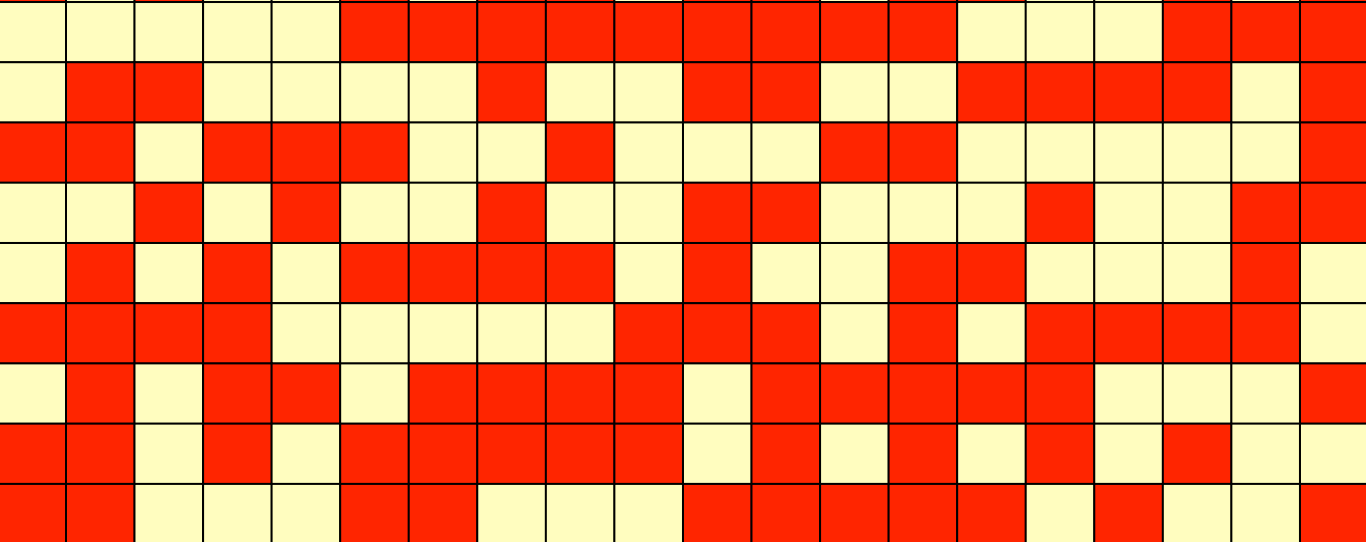
\includegraphics[width=\paperwidth]{Pic/Intro_pict.png}}
\title[AMS project]{ Stationary states of opinion diffusion}
\subtitle{Project for the exam: AMS (DSE)}
\author{Paola Serra and Marzio De Corato }
\date{\today}

\begin{document}

\begin{frame}
\vspace{+4 cm}  \titlepage
\end{frame}

\usebackgroundtemplate{ } 

% Uncomment these lines for an automatically generated outline.
%\begin{frame}{Outline}
%\setcounter{tocdepth}{1}
%\begin{center}
%  \tableofcontents
%\end{center}
%\end{frame}





\begin{frame}{}
\begin{center}
{\Huge Theoretical Framework}
\end{center}
\end{frame}


\section{Statistical Mechanics}

\begin{frame}{}
\begin{center}
{\Huge Statistical Mechanics}
\end{center}
\begin{center}
\textit{“Ludwig Boltzmann, who spent much of his life studying statistical mechanics, died in 1906, by his own hand. Paul Ehrenfest, carrying on the work, died similarly in 1933. Now it is our turn to study statistical mechanics.” States of Matter (1975), by David L. Goodstein}
\end{center}
\end{frame}

\begin{frame}{Concepts of statistical mechanics: entropy \cite{peliti2011statistical}}
\textbf{Central problem of thermodynamics:} characterize the actual state of equilibrium among all virtual states  \\
\textbf{Entropy postulate}: there exist a function S of the extensive variables $(X_{0},X_{1}...X_{r})$ called entropy,  that assumes the maximum value for a state of equilibrium among all vritual states and that possesses the following properties:
\begin{itemize}
\item Extensivity $S^{(1\cup2)}=S^{1}+S^{2}$
\item Convexity $S((1-\alpha)X^{1}+\alpha X^{2}) \geq (1-\alpha)S(x^{1})+\alpha S(X^{2})$
\item Monotonicity $\dfrac{\partial S}{\partial E}|_{X_{1}...X_{r}}=\frac{1}{T}>0$
\end{itemize}
\textbf The equilibrium state corresponds to the maximum entropy compatible with the constrains

\end{frame}


\begin{frame}{Concepts of statistical mechanics: entropy \cite{peliti2011statistical}}

\begin{itemize}
\item \textbf{Fundamental postulate of statistical mechanics} $S=k_{b}\ln|\Gamma|$
\item Where S is the thermodynamic entropy,  $k_{b}$ is Boltzmann constant and $|\Gamma|$ the volume in the phase space
\end{itemize}
\begin{equation}
\begin{split}
S(X_{0},...,X_{r})&=k_{b}\ln \int_{\Gamma}dx= \\
 & k_{b}\int dx\prod_{i=0}^{r}\left[\theta(X_{i}(x)-(X_{i}-\Delta X_{i}))\theta(X_{i}-X_{i}(x))\right]$
\end{split}
\end{equation}
\begin{itemize}
\item $(X_{0},...,X_{r})$ are the extensive variables
\item The $\theta$ functions assures that the integrand is not null only in the interval $X_{i} - \Delta X_{i} \leq X_{i}(x) \leq X_{i} $
\end{itemize}
\end{frame}

\begin{frame}{Concepts of statistical mechanics: micro-canonical ensamble}
\begin{itemize}
\item Lets focus on a particular observable A (extensive)
\end{itemize}
\begin{equation}
S(X;a)=k_{b}\ln\int_{\Gamma}dx\delta(A(x)-a)
\end{equation}

\begin{equation}
S(X)=S(X;a*)\geq S(X;a)
\end{equation}


\begin{equation}
\begin{split}
\frac{|\Gamma (a)|}{|\Gamma |}&=\frac{1}{|\Gamma |}\int_{\Gamma}dx\delta(A(x)-a)) \\
=& \exp\left\lbrace \frac{1}{k_{b}} \left[ S(X;a) - S(X;a^{*})\right] \right\rbrace \\
\simeq& \exp\left\lbrace   \dfrac{1}{k_{b}} \left[ \dfrac{\partial^{2}S}{\partial A^{2}}|_{a^{*}} (a-a^{*})^{2} \right] \right\rbrace
\end{split}
\end{equation}

\begin{equation}
a^{*}=\left\langle A(x) \right\rangle =\frac{1}{|\Gamma|}\int_{\Gamma}dx A(x)
\end{equation}

\end{frame}

\begin{frame}{Concepts of statistical mechanics: canonical ensemble}
\begin{equation}
a^{*}=\frac{1}{|\Gamma|}\int_{\Gamma}dx_{s}dx_{R} A(x_{s})
\end{equation}
\begin{equation}
\left\langle A(x) \right\rangle=\int dx_{s}dx_{r}A(x_{S})\delta(H^{(s)})
\end{equation}
\begin{equation}
\left\langle A(x) \right\rangle=\frac{1}{|\Gamma|}\int dx_{s}dx_{r}A(x_{s})\delta(H^{S}(x_{s})+H^{R}(x_{R})-H^{S}(x_{S}))
\end{equation}
\begin{equation}
\left\langle A(x) \right\rangle=\frac{1}{|\Gamma|}\int  dx_{s}A(x_{s})\times\int dx_{r}\delta(H^{R}(x_{R})-(E-H^{(S)}(x_{s})))
\end{equation}
\begin{equation}
\int dx_{r}\delta(H^{R}(x_{R})-(E-H^{(S)}(x_{s})))\simeq \exp\left\lbrace\frac{1}{k_{b}} S^{R}(E-H^{S})\right\rbrace
\end{equation}


\end{frame}


\begin{frame}{Concepts of statistical mechanics: canonical ensemble}

\begin{equation}
\exp\left\lbrace\frac{1}{k_{b}} S^{R}(E-H^{S})\right\rbrace \simeq  \exp \left[ \frac{1}{k_{b}}S^{R}(E)      \right] \exp\left[  -\frac{1}{k_{b}}\frac{\partial S^{(R)}}{\partial E}|_{E}  H^{(S)}(x_{S})  \right]
\end{equation}

\begin{equation}
\left\langle A(x) \right\rangle=\dfrac{1}{Z}\int dx_{s}A(x_{s})exp\left[ -\frac{H^{(S)}(x_{s})}{k_{b}T} \right]
\end{equation}

\begin{equation}
Z=\int dx_{s}exp\left[  -\frac{H^{S}(x_{s})}{k_{b}T}  \right]
\end{equation}


\begin{equation}
\left\langle A(x) \right\rangle=\dfrac{1}{Z}\int dE\int dx\delta(H(x)-E)A(x)exp(-\dfrac{E}{k_{b}T})
\end{equation}

\begin{equation}
\left\langle A(x) \right\rangle=\dfrac{1}{Z}\int dE'a^{*}(E')exp\left[ - \dfrac{E'-TS(E')}{k_{b}T}\right]
\end{equation}


\end{frame}


\begin{frame}{Concepts of statistical mechanics: canonical ensemble\cite{peliti2011statistical} }

\begin{equation}
Z\simeq \exp\left[-\dfrac{E^{*}-TS(E^{*})}{k_{b}T} \right]=\exp\left( - \frac{F}{k_{b}T}  \right)     
\end{equation}

\begin{equation}
\dfrac{\partial ln Z(\beta)}{\partial \beta}=-\dfrac{1}{Z}\int dx H(x)\exp\left[  -\dfrac{H}{k_{b}T}\right]=-\left\langle H(x) \right\rangle=-E
\end{equation}

\begin{equation}
\dfrac{\partial^{2} ln Z(\beta)}{\partial \beta^{2}}=\left\langle H(x)^{2} \right\rangle-\left\langle H(x) \right\rangle^{2}
\end{equation}

\begin{equation}
\left\langle H(x)^{2} \right\rangle-\left\langle H(x) \right\rangle^{2}=-\dfrac{\partial E}{\partial (1/k_{b}T)}=k_{b}T^{2}\dfrac{\partial E}{\partial T}=k_{b}T^{2}C
\end{equation}

In this way a statistical quantity the variance has been connected to a thermodynamic quantity: the temperature.

\end{frame}

\section{Ising model}

\begin{frame}{}
\begin{center}
{\Huge Ising Model}
\end{center}
\end{frame}


\begin{frame}{Ising model \cite{mackay2003information,slides}}
\begin{itemize}
\item An array of atoms that can take states $\pm 1$
\item $E(\textbf{x},J,H)= - \left[\dfrac{1}{2}\sum_{m,n}J_{mn}x_{m}x_{n}+\sum_{n}Hx_{n} \right]$
\item $P(x|\beta,J,H)=\frac{1}{Z(\beta,J,H)}\exp[-\beta E(x,J,H)]$
\item $\beta=1/k_{b}T\quad Z(\beta,J,H)=\sum_{x}exp\left[-\beta E(x,J,H)\right]$
\item $g(m)=\frac{\left\langle \sigma_{i}\sigma_{i+m}  \right\rangle - \left\langle \sigma_{i} \right\rangle \left\langle \sigma_{i+m} \right\rangle  }{1- \left\langle \sigma_{i} \right\rangle \left\langle \sigma_{i+m} \right\rangle }=\left\langle \sigma_{i}\sigma_{i+m}  \right\rangle $ if $H=0$
\end{itemize}
\end{frame}

\section{Numerical simulation}

\begin{frame}{}
\begin{center}
{\Huge Numerical simulations}
\end{center}
\begin{center}
\textit{“Never make a calculation until you know the answer. Make an estimate before every calculation, try a simple physical argument (symmetry! invariance! conservation!) before every derivation, guess the answer to every paradox and puzzle. Courage: No one else needs to know what the guess is. Therefore make it quickly, by instinct. A right guess reinforces this instinct. A wrong guess brings the refreshment of surprise. In either case life as a spacetime expert, however long, is more fun!” John Archibald Wheeler }
\end{center}
\end{frame}


\begin{frame}{Numerical simulation \cite{peliti2011statistical}}
\begin{itemize}
\item \textbf{Simulation} \textit{the evolution equations of a system are defined to such a detail that a computer can make its behaviour explicit, and one looks to see what takes place} 
\item Numerical experiment 
\item \textbf{Molecular dynamics:} the equation of motion are solved numerically PROS: information of both the dynamical and static properties of the system are explored 
\item\textbf{Monte Carlo:} a fictitious evolution process of the system is solved in order to get the equilibrium distribution PROS  1) also the systems whose dynamics is not defined can be explored 2) a fictitious dynamics can be considered in order to reach the equilibrium faster 
\item Molecular dynamics may provide a proof of statistical mechanics, Monte Carlo methods presuppose its validity
\end{itemize}
\end{frame}


\begin{frame} {Monte Carlo method \cite{peliti2011statistical}}

 \begin{center}
     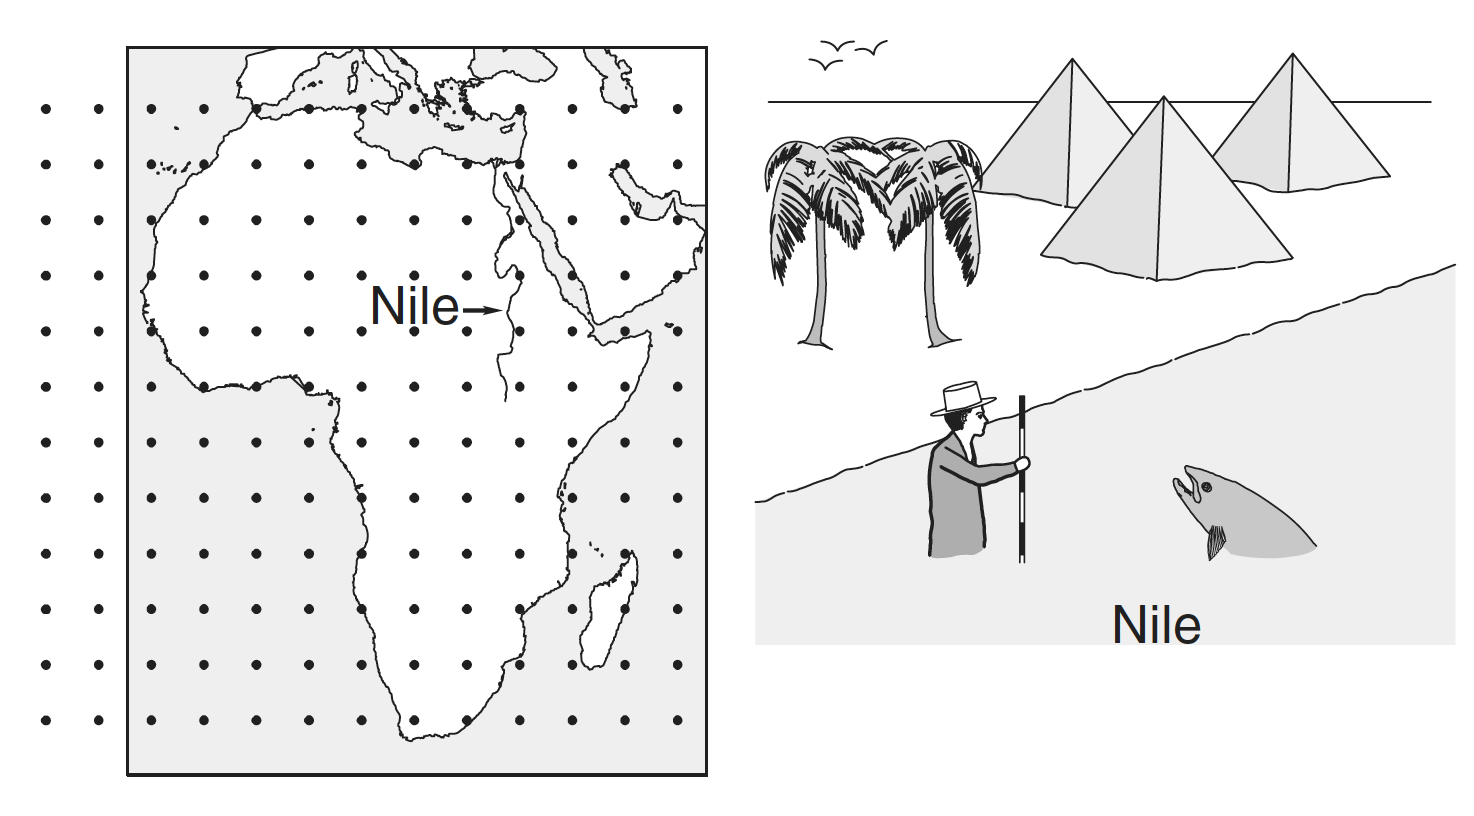
\includegraphics[width=0.7\textwidth]{Pic/Pic_river.png}
\end{center}

\end{frame}


\begin{frame}{Monte Carlo method \cite{peliti2011statistical}}


\begin{itemize}
\item We would calculate an integral of type $\left\langle  A\right\rangle = \int^{1}_{0} dxA(x)\rho(x)$ where $\rho$ is the probability distribution.



\item Evaluate the integrand in N+1 points uniformly arranged between 0 and 1  $\left\langle  A\right\rangle \approx \frac{1}{N+1}\sum_{i=0}^{N}A(x_{i})\rho(x_{i})$



\item A better convergence is reached if the $x_{i}$ density is proportional to $\rho(x)$.  In this case we have $\left\langle  A\right\rangle = 1/N\sum_{i=1}^{N}A(\textbf{x}_{i})$.  


\end{itemize}
\end{frame}







\begin{frame}{Monte Carlo method \cite{peliti2011statistical}}

\begin{itemize}

\item The quantity $\left\langle  A\right\rangle $ is evaluated over a distribution $\rho(x)$ where $x_{i}$ are random,  independent and distributed with a probability density $\rho(x)$



\item The independence conditions can be relaxed with the condition that the correlations between $x_{i}$ and $x_{i+l}$ go to zero fairly rapidly as l grows 


\item The true dynamics is replaced with a fictitious stochastic dynamics.  The state at $t+1$ depends only from the state at $t$.  $\rightarrow$ Markov Chain 

\end{itemize}

\end{frame}

\begin{frame}{Monte Carlo method \cite{peliti2011statistical}}

\begin{itemize}

\item The evolution of probability is described by the \textbf{master equation} $\Delta p_{a}(t)=\sum'_{b\neq a}[W_{ab}p_{b}(t)-W_{ba}p_{a}(t)]$


\item stationary  \rightarrow $ \sum'_{b\neq a}[W_{ab}p_{b}(t)-W_{ba}p_{a}(t)=0\quad \forall a$


\item Detailed balance property $W_{ab}W_{bc}W_{ca}=W_{ac}W_{cb}W_{ba}$


\item $ W_{ab}p_{b}(t)-W_{ba}p_{a}(t)=0\quad \forall a,b$
\end{itemize}

\end{frame}


\begin{frame}{Monte Carlo method \cite{peliti2011statistical}}

\begin{itemize}

\item We would sample $p^{eq}_{a}$ 

\item This can be performed as long as the $W_{ab}$ is ergodic and the detailed balance property holds 

\item The transition between any two arbitrary states can take place as long as one waits for a sufficient amount of time

\end{itemize}

\end{frame}

\begin{frame}{Application \cite{peliti2011statistical}}

\begin{itemize}
\item $H(\sigma)=-\sum_{\left\langle ij \right\rangle}J\sigma_{i}\sigma_{j}-\sum_{i}h\sigma_{i}$
\item $P_{\sigma}=\frac{e^{-H(\sigma)/k_{b}T}}{Z}$  $\quad Z=\sum_{\sigma}e^{-H(\sigma)/k_{b}T}$
\item The observable are calculated as $E=\left\langle H \right\rangle=\sum_{sigma}H(\sigma)P_{\sigma'}^{B} \quad M=\sum_{\sigma}\left(\sigma_{i} \sigma\right)P_{\sigma}^{B}  $
\item The markov chain states should be the microstates $\sigma$ and $P_{\sigma}$ the stationary distribution 
\item $W_{\sigma\sigma '} = W_{\sigma ' \sigma}$ $\dfrac{P_{\sigma}}{P_{\sigma '}}=W_{\sigma ' \sigma} \exp - \dfrac{H(\sigma)-H(\sigma ')}{k_{b}T}$
\item The Z term is no more present !!!
\end{itemize}

\end{frame}

\begin{frame}{Application \cite{peliti2011statistical}}

\begin{itemize}
\item $W_{\sigma' \sigma }= \begin{cases} 
\kappa  H(\sigma ') <  H(\sigma )  \\ 
\kappa\exp\left\lbrace -\left[ H(\sigma ')-H(\sigma) \right] / k_{b}T \right\rbrace$ \end{cases}
\item $\left\lbrace A \right\rbrace \neq \left[  A \right]_{T}=\frac{1}{T}$
\item $A(\sigma)=\left\langle  A \right\rangle \left[1+O(N^{-1/2})\right] \forall \sigma \in \Gamma $  
\item $S=0.5Nk_{b}ln2 \quad \dfrac{|\Gamma|}{2^{N}}\approx 2^{-0.5N}\quad N=100 \quad 10^{-15}$
\item $ \approx \left[ A \right]_{T}=\dfrac{1}{T}\sum^{T\left\langle A  \right\rangle_{0}+T}_{t=T_{0}}A_{\sigma(t)} $
\item $\left\langle \Delta A_{T}^{2}  \right\rangle \approx \dfrac{1}{T}\left(A_{\sigma(t)}-\left[A\right]_{T} \right)^{2}$ 
\item $\sigma_{t}$ and $\sigma_{t'}$ are indipendent if $|t-t'|$ is larger that a characteristic time $\tau_{0}$
\item   $\left\langle \Delta A_{T}^{2}  \right\rangle \approx \dfrac{\tau_{0}}{T}\left(A_{\sigma(t)}-\left[A\right]_{T} \right)^{2}$


\end{itemize}

\end{frame}


\section{Goals and methods}

\begin{frame}
\begin{center}
{\Huge Goals and methods}
\end{center}
\end{frame}

\begin{frame}{Goals and methods}
\begin{itemize}
\item Reproduce the main result for a 2D anti ferromagnetic lattice $(J=-1)$ with no external magnetic field $(H=0)$ with the montecarlo-metropolis
\item  Once checked that the script provide the correct results apply it to a lattice $(J=+1)$.  In this case the spins represent an opinion and the sites people.  The goal is to find the stationary states (at $T=0$ and $T\neq0$)
\item Introduce in the lattice some blocks that never change their status.  These islands represent groups that never change mind and only diffuse their ideas.  (at $T=0$ and $T\neq0$)
\end{itemize}
\end{frame}

\section{Results}

\begin{frame}
\begin{center}
{\Huge Results}
\end{center}
\end{frame}

\begin{frame}{Simulation features}
\begin{itemize}
\item 10x10 lattice 
\item Periodic boundary conditions $\rightarrow$ the topology of a torus (genus equal to 1) 
\item 6000 steps 
\end{itemize}
\begin{columns}
\begin{column}{0.5\textwidth}
    \begin{center}
     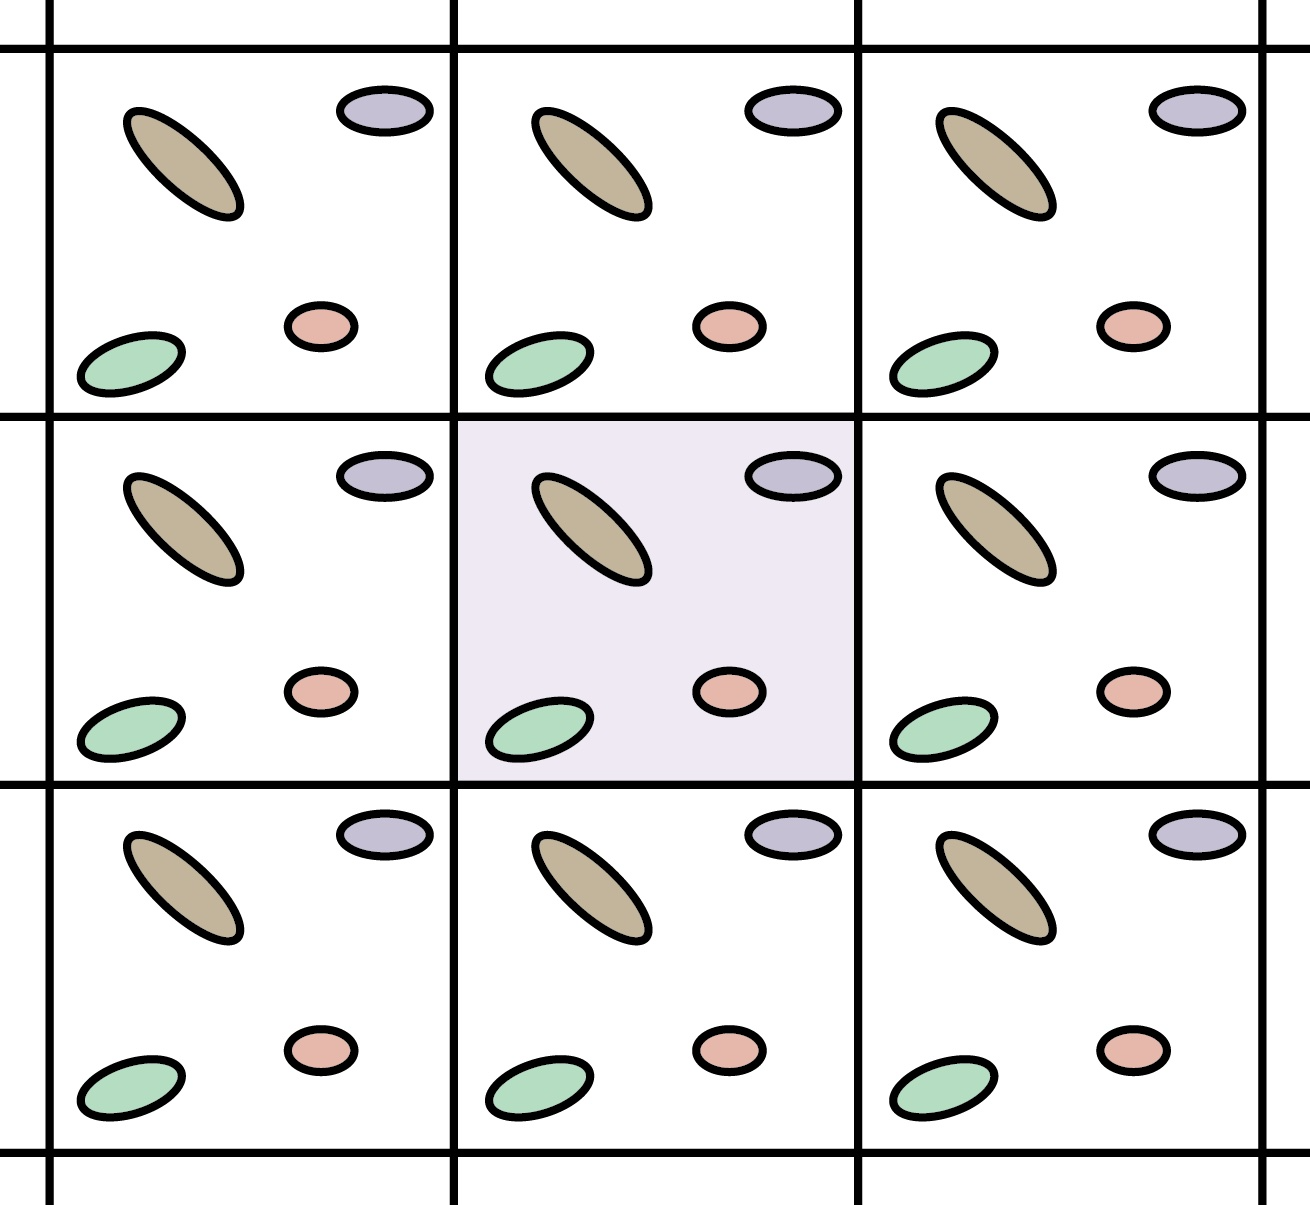
\includegraphics[width=0.7\textwidth]{Pic/PBC.png}
      \end{center}
      \begin{center}
          Image taken from \cite{PBC}
     \end{center}
\end{column}
\begin{column}{0.5\textwidth}

    \begin{center}
     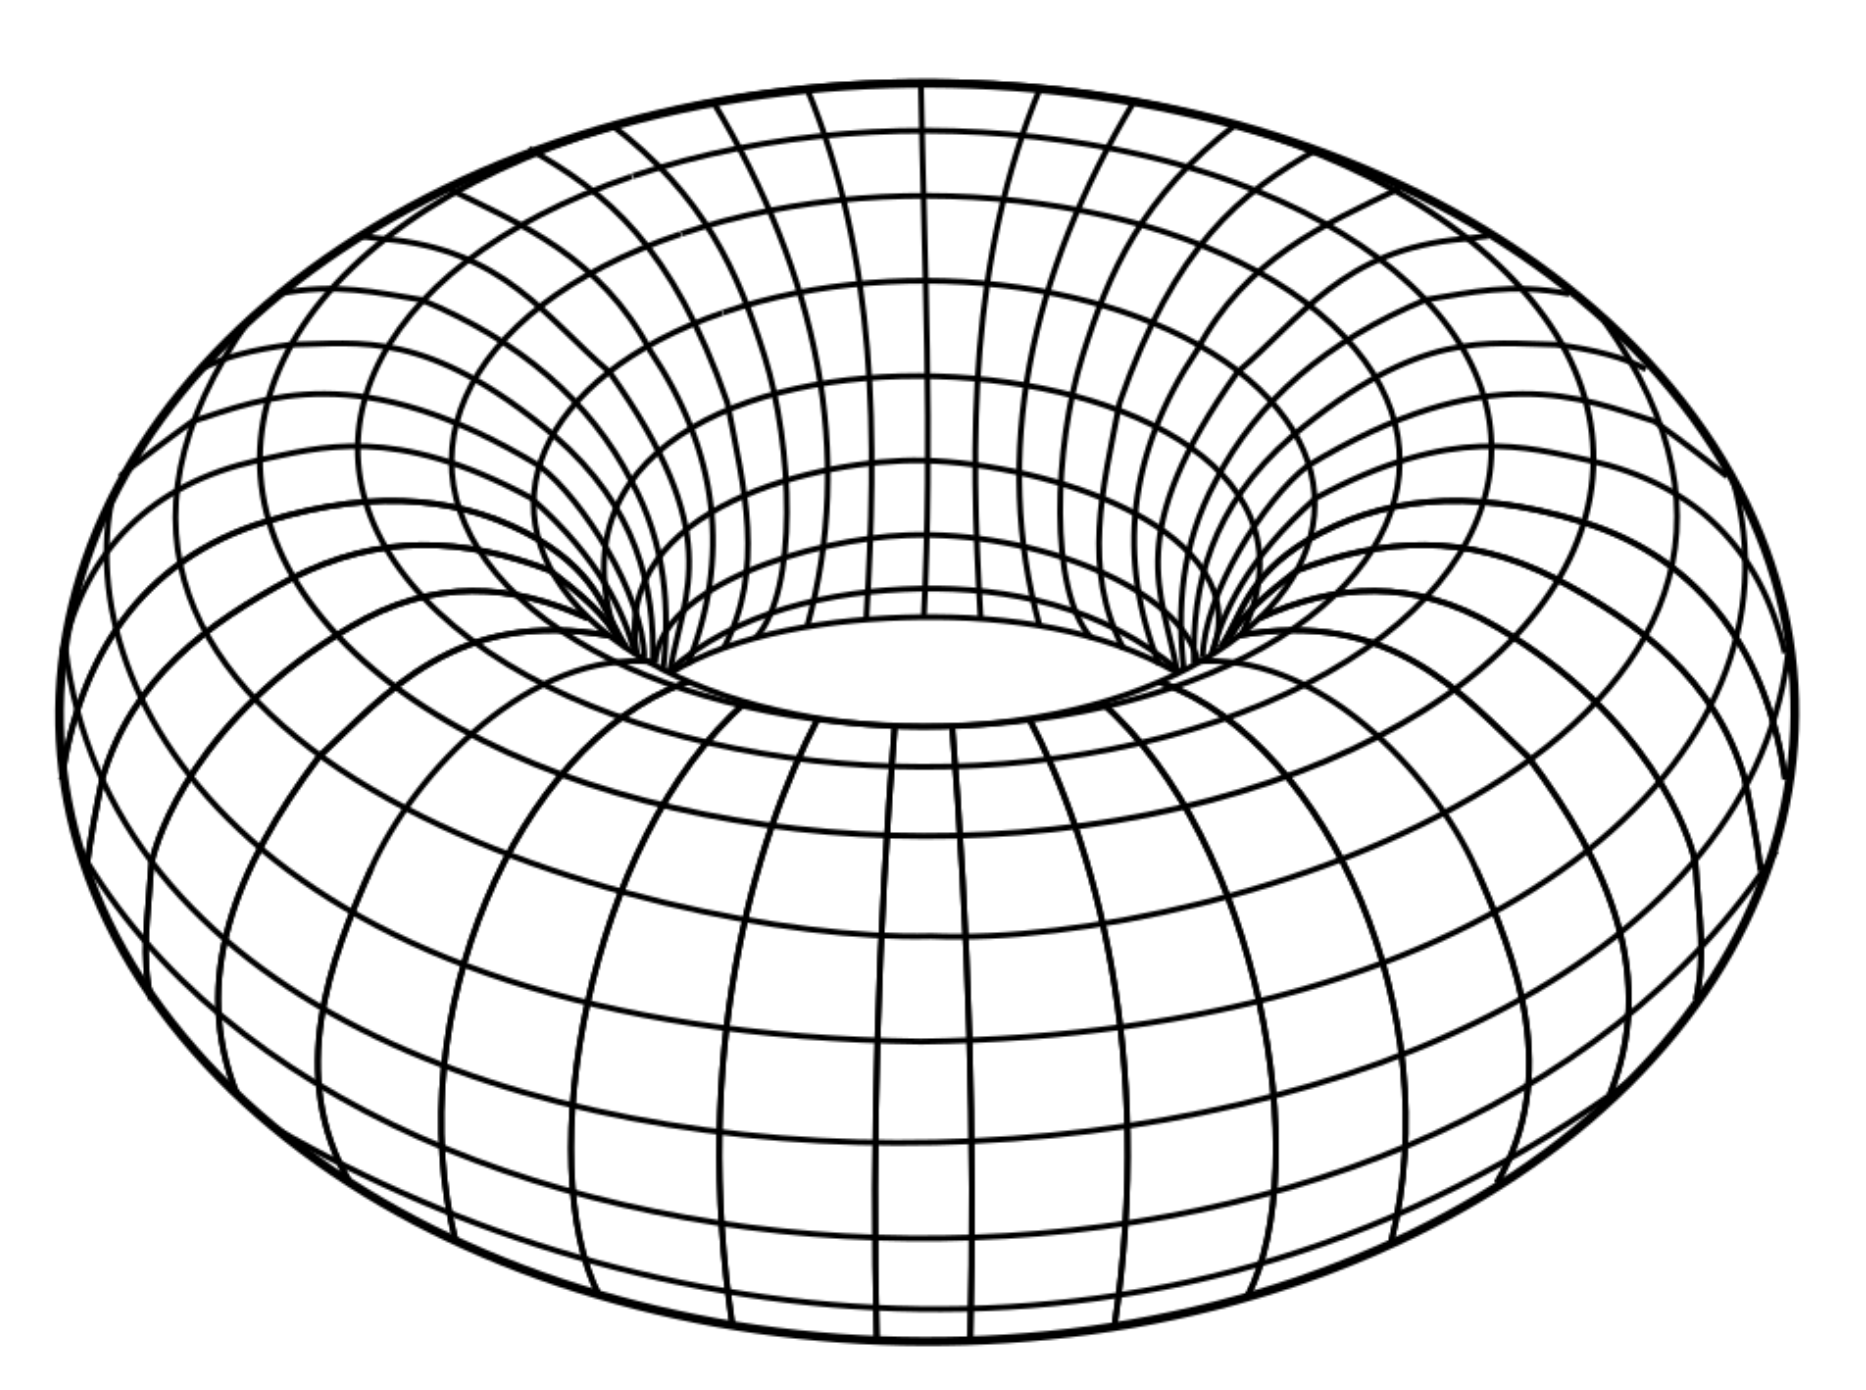
\includegraphics[width=0.7\textwidth]{Pic/Torus.png}
      \end{center}
      \begin{center}
          Image taken from \cite{PBC}
     \end{center}

\end{column}
\end{columns}
\end{frame}


\subsection{Antiferromagnetic}


\begin{frame}{Antiferromagnetic J=-1, T=0}
\begin{columns}
\begin{column}{0.5\textwidth}
    \begin{center}
     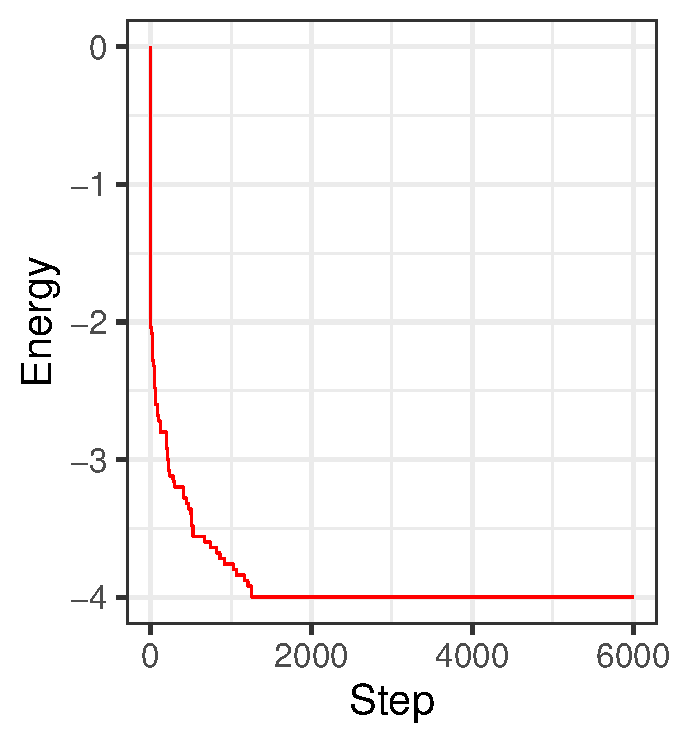
\includegraphics[width=\textwidth]{Pic/J-1_10_6000_T=0_ENERGY.pdf}
     \end{center}
\end{column}
\begin{column}{0.5\textwidth}
    \begin{center}
     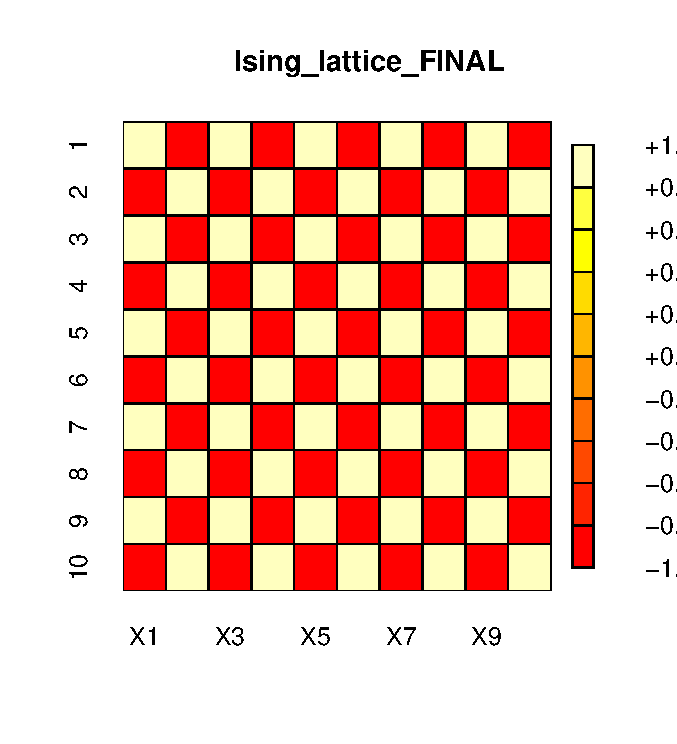
\includegraphics[width=\textwidth]{Pic/J-1_10_6000_T=0_FINAL.pdf}
     \end{center}
\end{column}
\end{columns}
\end{frame}

\begin{frame}{Antiferromagnetic J=-1, T=0}
\begin{columns}
\begin{column}{0.5\textwidth}
    \begin{center}
     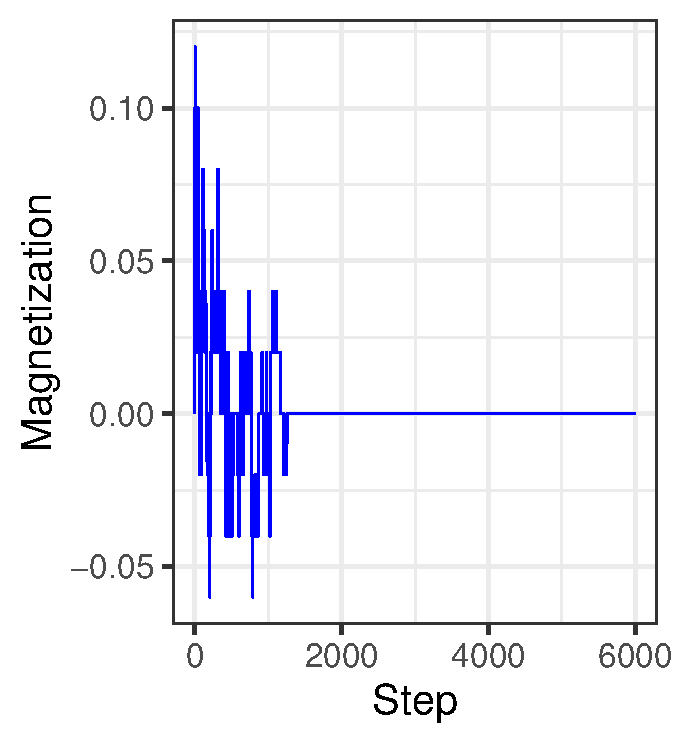
\includegraphics[width=\textwidth]{Pic/J-1_10_6000_T=0_Magnetization.pdf}
     \end{center}
\end{column}
\begin{column}{0.5\textwidth}
    \begin{center}
     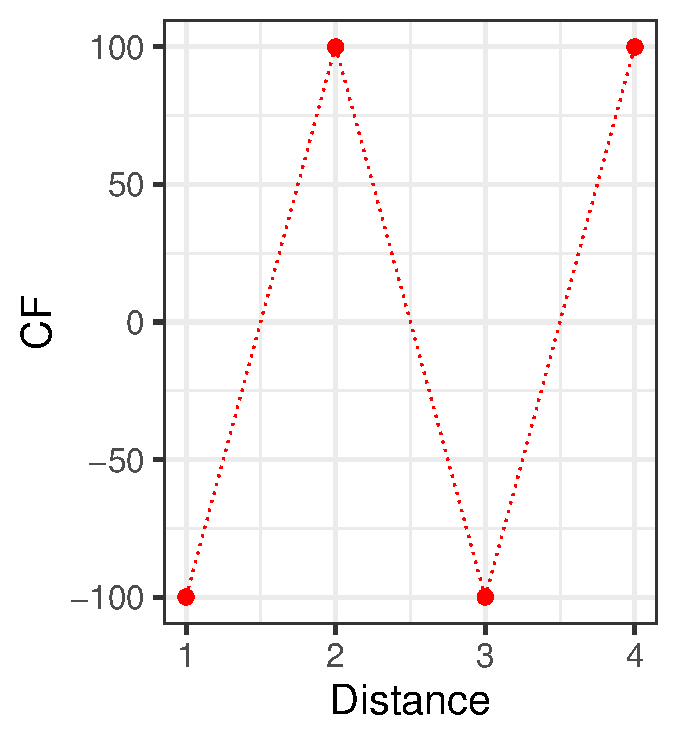
\includegraphics[width=\textwidth]{Pic/J-1_10_6000_T=0_CORRELATION.pdf}
     \end{center}
\end{column}
\end{columns}
\end{frame}


\begin{frame}{Antiferromagnetic J=-1, T=1.5}
\begin{columns}
\begin{column}{0.5\textwidth}
    \begin{center}
     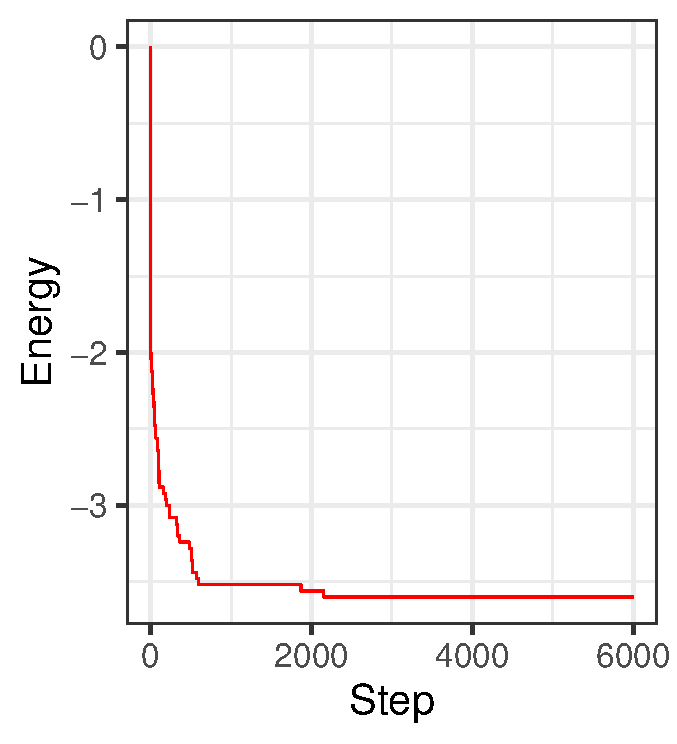
\includegraphics[width=\textwidth]{Pic/J-1_60_2500_T=1.5_ENERGY.pdf}
     \end{center}
\end{column}
\begin{column}{0.5\textwidth}
    \begin{center}
     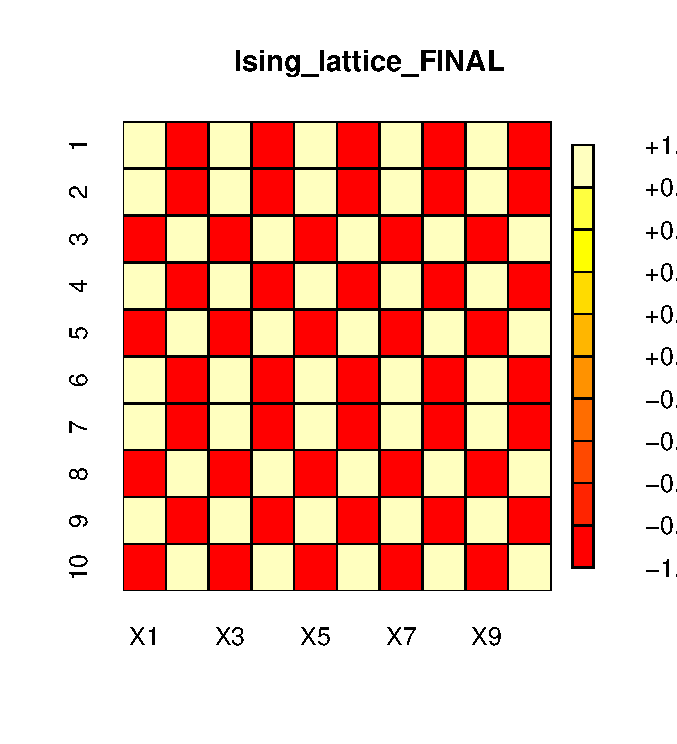
\includegraphics[width=\textwidth]{Pic/J-1_60_2500_T=1.5_FINAL.pdf}
     \end{center}
\end{column}
\end{columns}
\end{frame}

\begin{frame}{Antiferromagnetic J=-1, T=1.5}
\begin{columns}
\begin{column}{0.5\textwidth}
    \begin{center}
     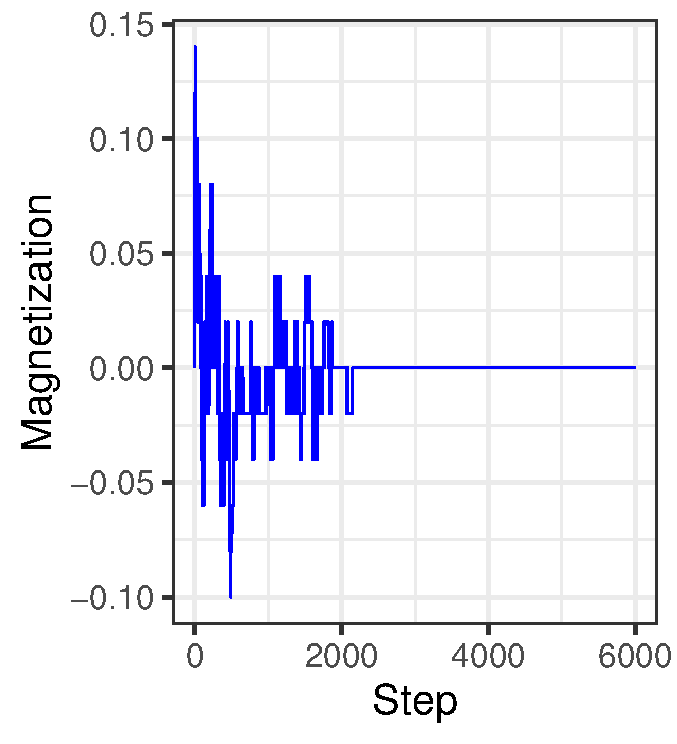
\includegraphics[width=\textwidth]{Pic/J-1_60_2500_T=1.5_Magnetization.pdf}
     \end{center}
\end{column}
\begin{column}{0.5\textwidth}
    \begin{center}
     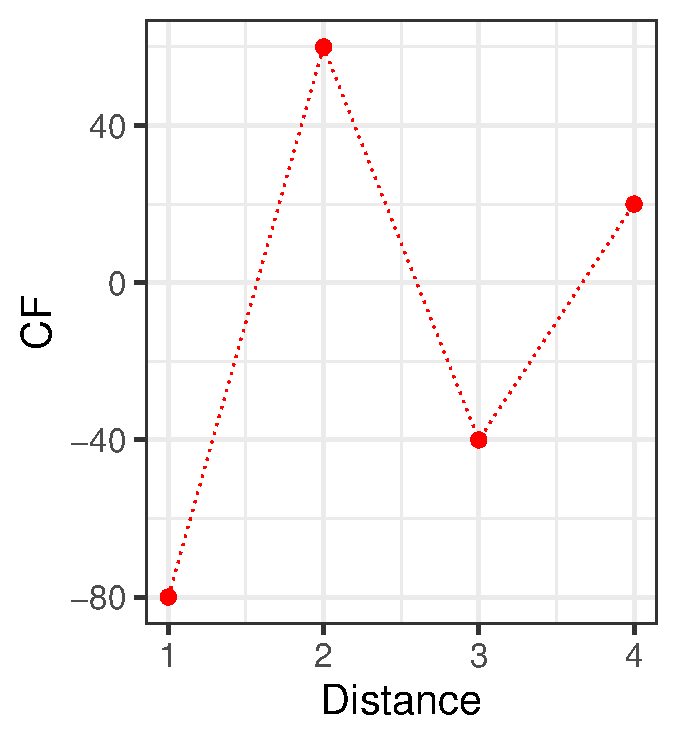
\includegraphics[width=\textwidth]{Pic/J-1_60_2500_T=1.5_CORRELATION.pdf}
     \end{center}
\end{column}
\end{columns}
\end{frame}

\begin{frame}{Antiferromagnetic J=-1, T=4}
\begin{columns}
\begin{column}{0.5\textwidth}
    \begin{center}
     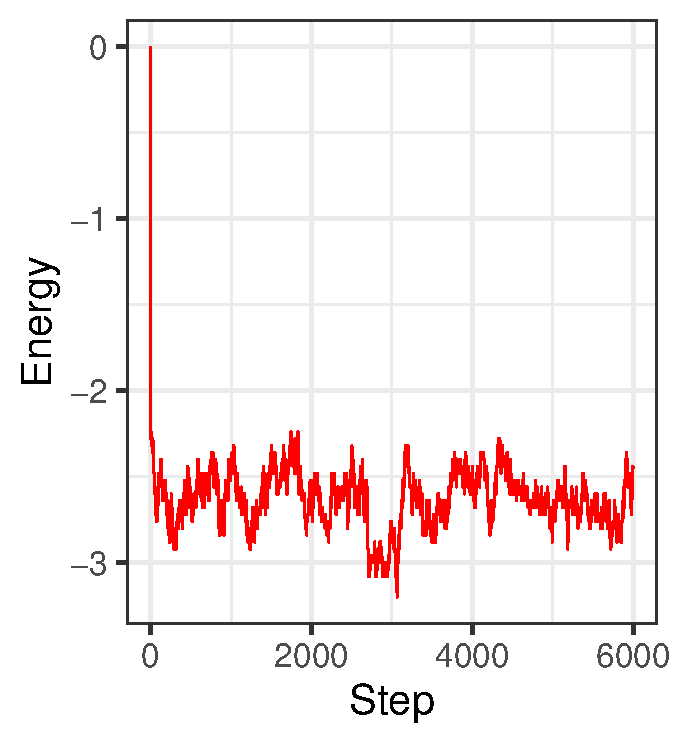
\includegraphics[width=\textwidth]{Pic/J-1_60_2500_T=4_ENERGY.pdf}
     \end{center}
\end{column}
\begin{column}{0.5\textwidth}
    \begin{center}
     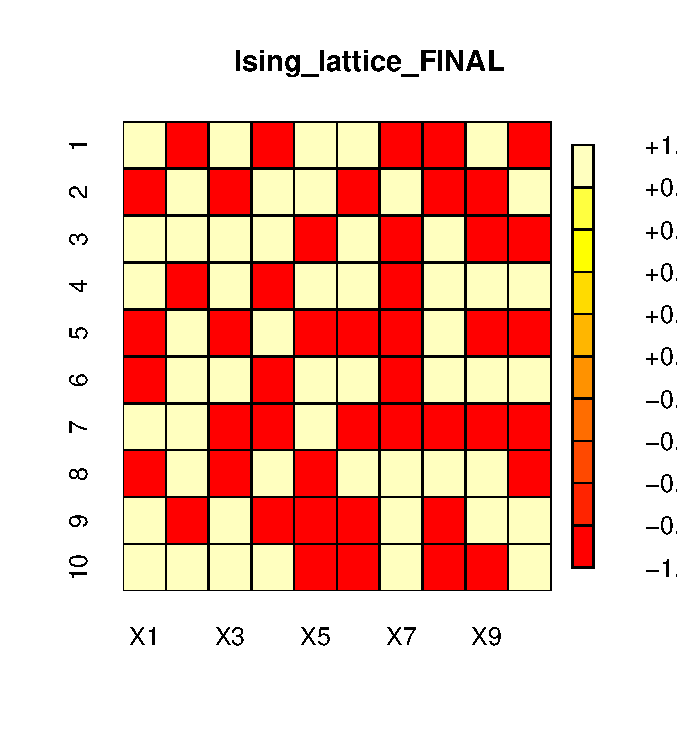
\includegraphics[width=\textwidth]{Pic/J-1_60_2500_T=4_FINAL.pdf}
     \end{center}
\end{column}
\end{columns}
\end{frame}

\begin{frame}{Antiferromagnetic J=-1, T=4}
\begin{columns}
\begin{column}{0.5\textwidth}
    \begin{center}
     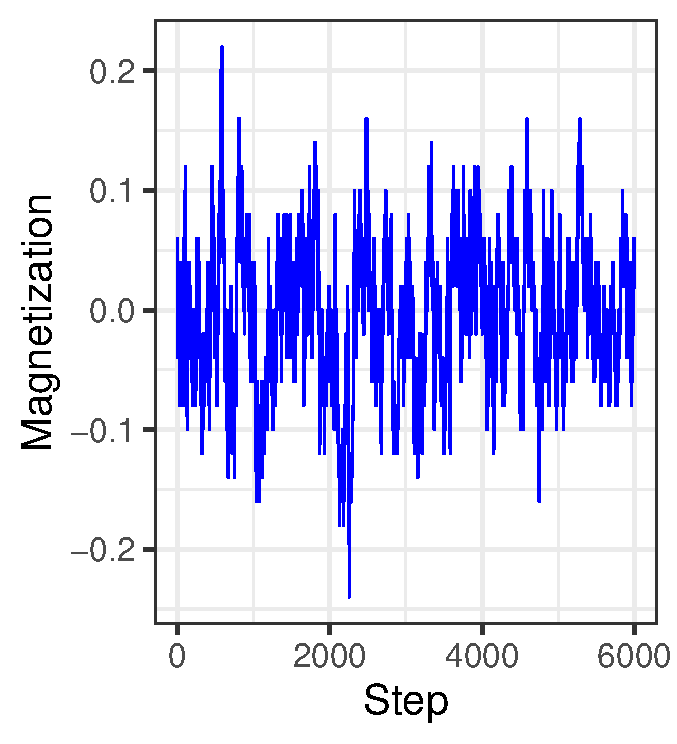
\includegraphics[width=\textwidth]{Pic/J-1_60_2500_T=4_Magnetization.pdf}
     \end{center}
\end{column}
\begin{column}{0.5\textwidth}
    \begin{center}
     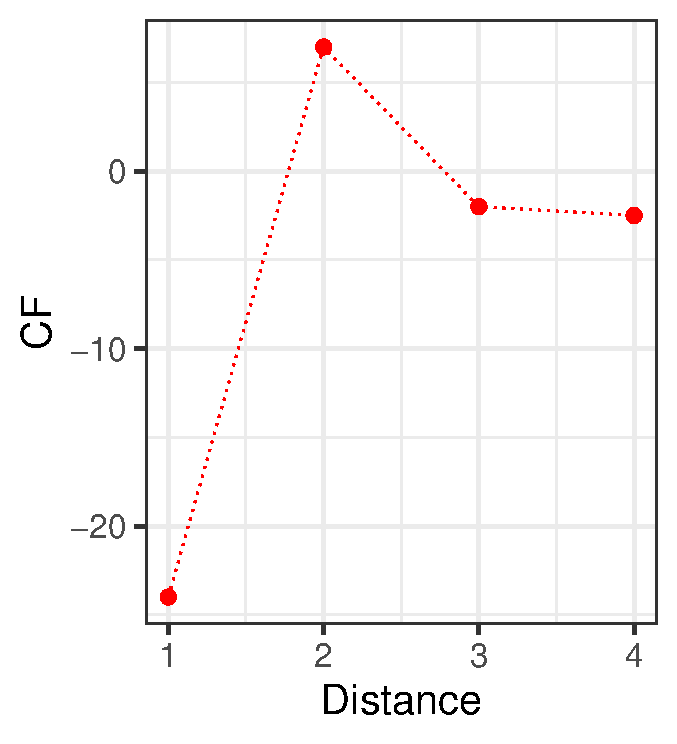
\includegraphics[width=\textwidth]{Pic/J-1_60_2500_T=4_CORRELATION.pdf}
     \end{center}
\end{column}
\end{columns}
\end{frame}


\begin{frame}{Antiferromagnetic J=-1, T=8}
\begin{columns}
\begin{column}{0.5\textwidth}
    \begin{center}
     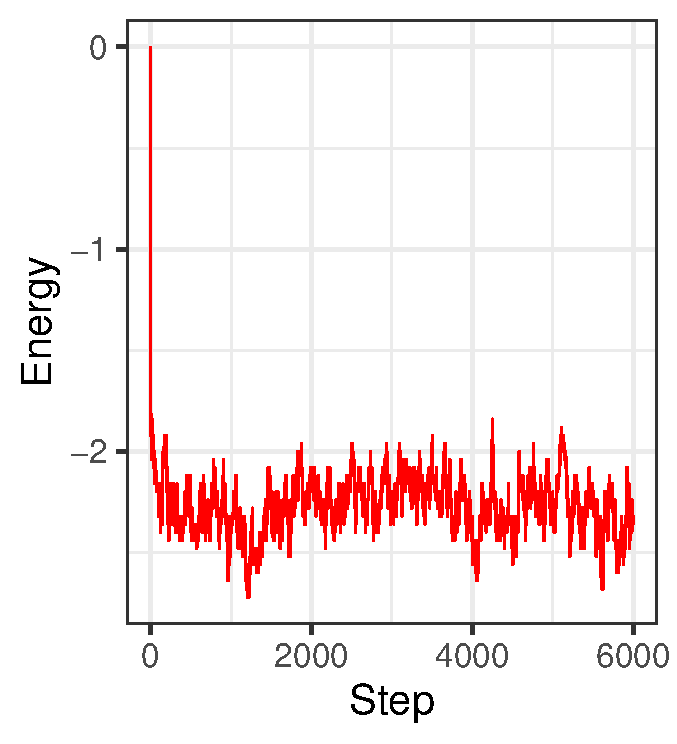
\includegraphics[width=\textwidth]{Pic/J-1_60_2500_T=8_ENERGY.pdf}
     \end{center}
\end{column}
\begin{column}{0.5\textwidth}
    \begin{center}
     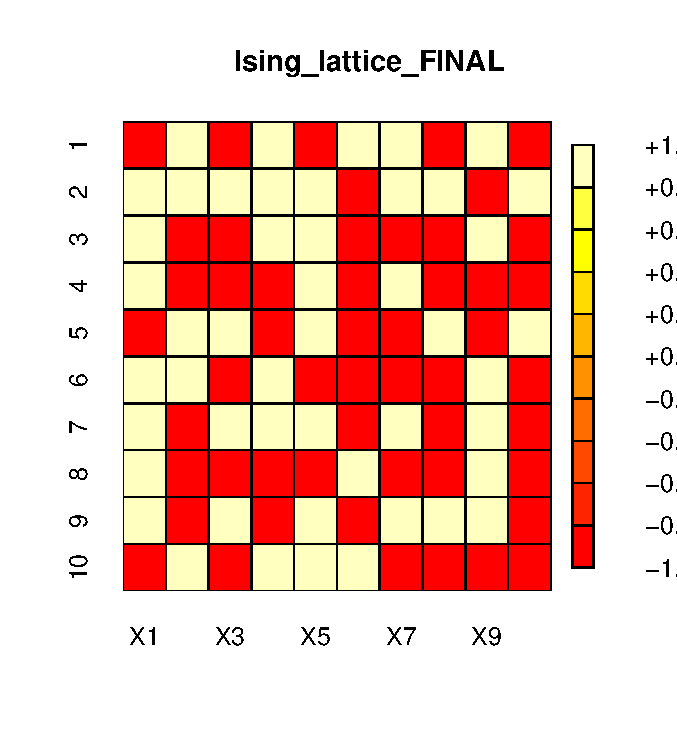
\includegraphics[width=\textwidth]{Pic/J-1_60_2500_T=8_FINAL.pdf}
     \end{center}
\end{column}
\end{columns}
\end{frame}

\begin{frame}{Antiferromagnetic J=-1, T=8}
\begin{columns}
\begin{column}{0.5\textwidth}
    \begin{center}
     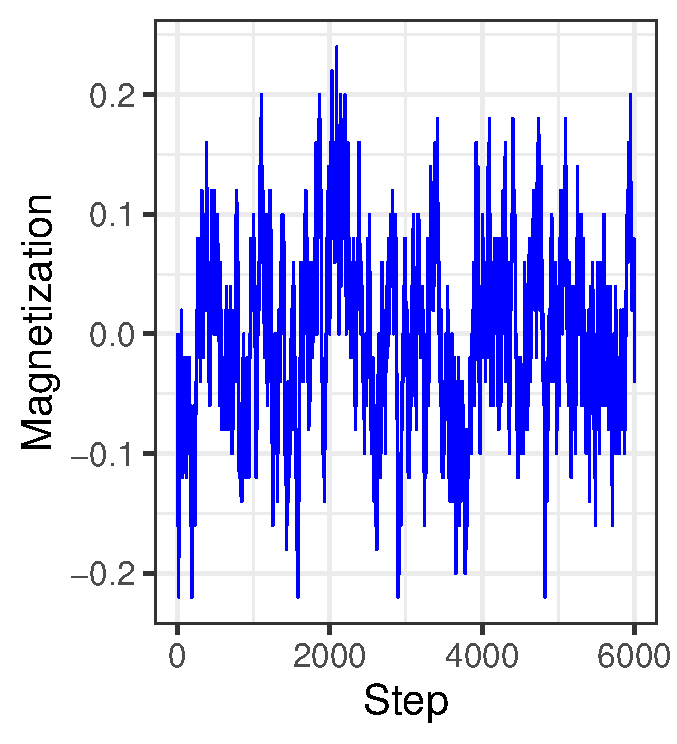
\includegraphics[width=\textwidth]{Pic/J-1_60_2500_T=8_Magnetization.pdf}
     \end{center}
\end{column}
\begin{column}{0.5\textwidth}
    \begin{center}
     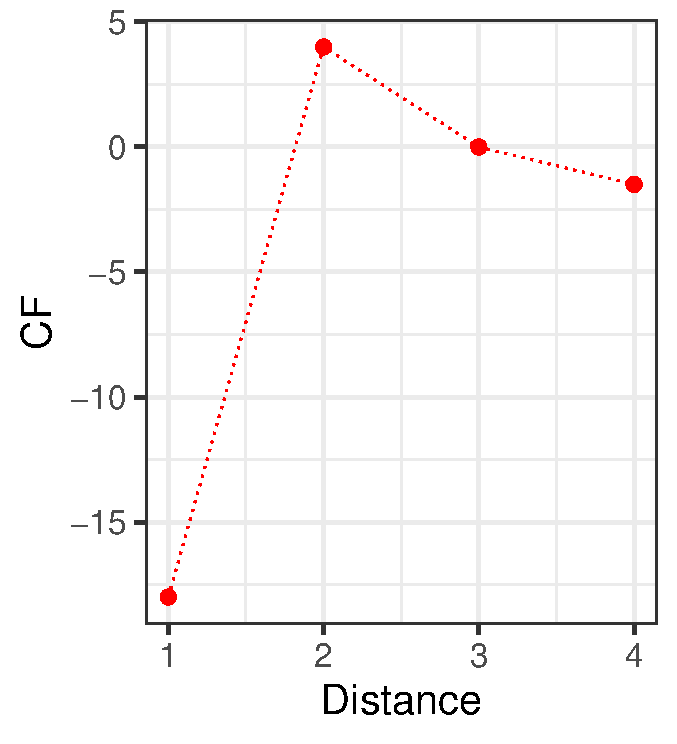
\includegraphics[width=\textwidth]{Pic/J-1_60_2500_T=8_CORRELATION.pdf}
     \end{center}
\end{column}
\end{columns}
\end{frame}

\subsection{Ferromagnetic}

\begin{frame}{Ferromagnetic J=-1, T=30}
\begin{columns}
\begin{column}{0.5\textwidth}
    \begin{center}
     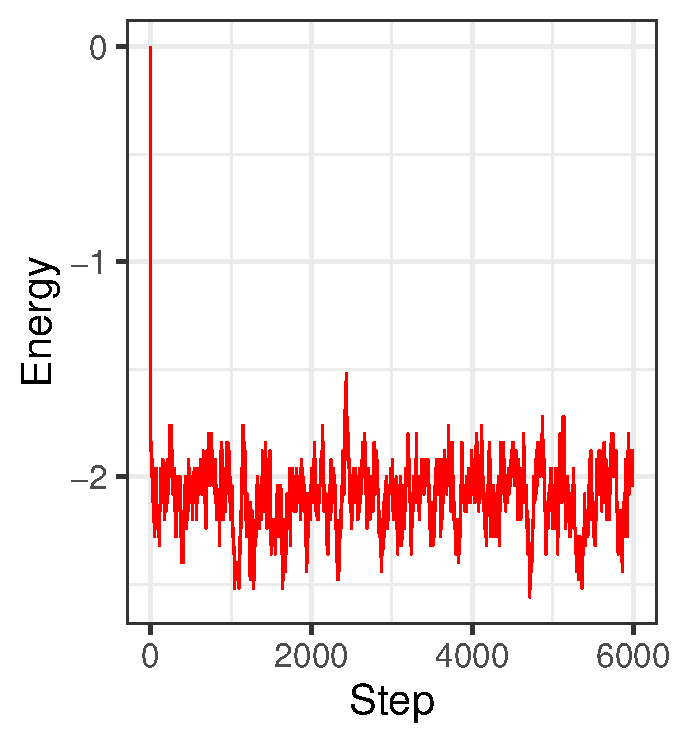
\includegraphics[width=\textwidth]{Pic/J-1_10_6000_T=30_ENERGY.pdf}
     \end{center}
\end{column}
\begin{column}{0.5\textwidth}
    \begin{center}
     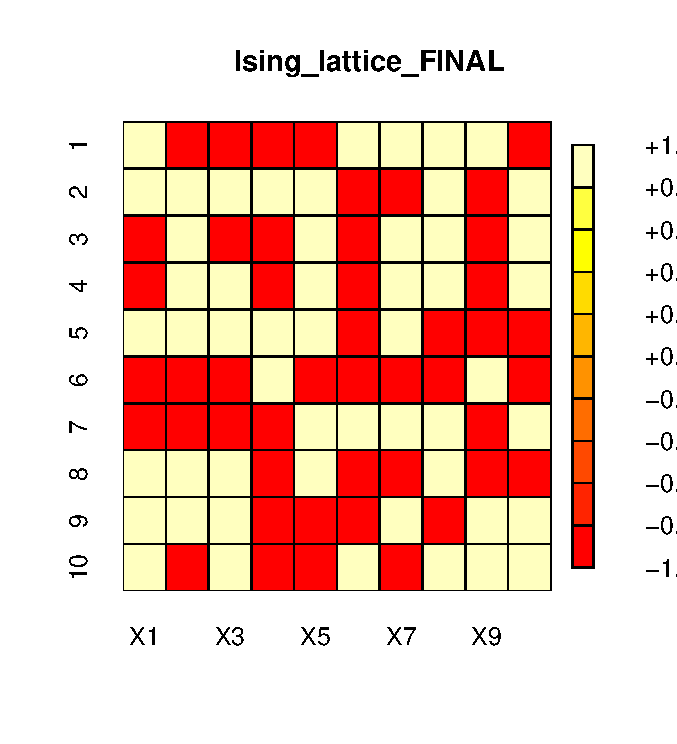
\includegraphics[width=\textwidth]{Pic/J-1_10_6000_T=30_FINAL.pdf}
     \end{center}
\end{column}
\end{columns}
\end{frame}

\begin{frame}{Ferromagnetic J=-1, T=30}
\begin{columns}
\begin{column}{0.5\textwidth}
    \begin{center}
     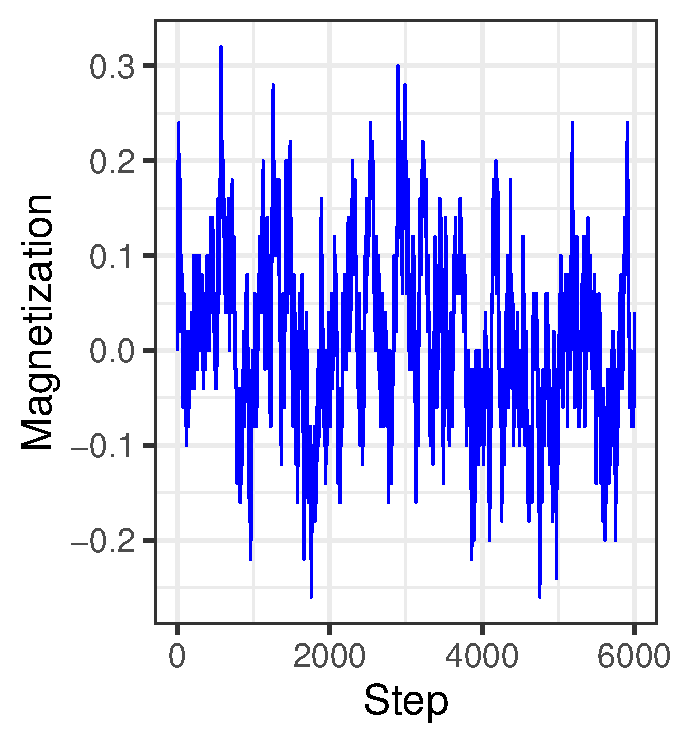
\includegraphics[width=\textwidth]{Pic/J-1_10_6000_T=30_Magnetization.pdf}
     \end{center}
\end{column}
\begin{column}{0.5\textwidth}
    \begin{center}
     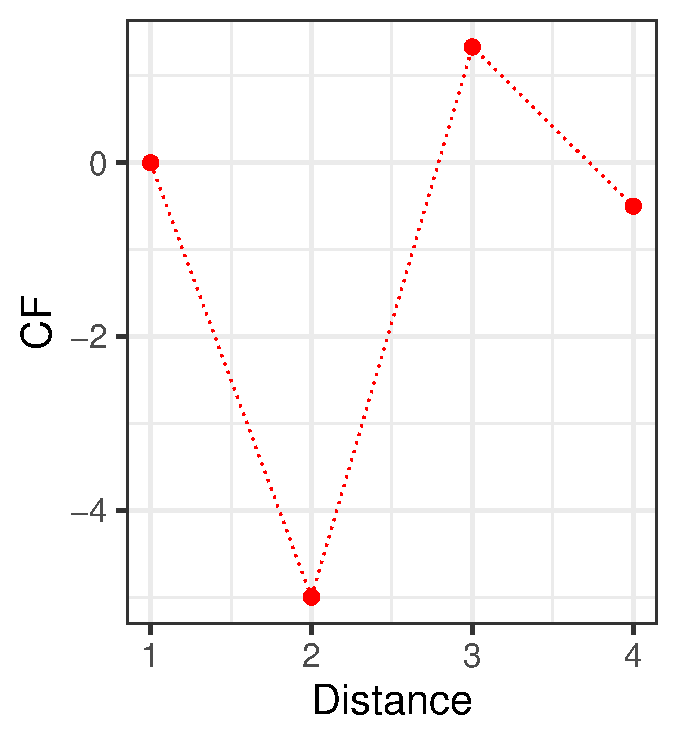
\includegraphics[width=\textwidth]{Pic/J-1_10_6000_T=30_CORRELATION.pdf}
     \end{center}
\end{column}
\end{columns}
\end{frame}

\begin{frame}{Ferromagnetic J=+1, T=0}
\begin{columns}
\begin{column}{0.5\textwidth}
    \begin{center}
     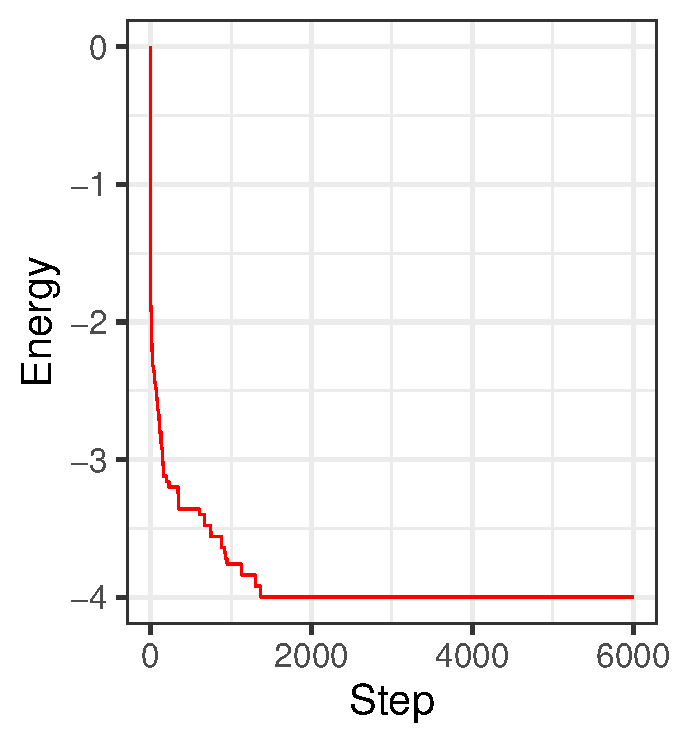
\includegraphics[width=\textwidth]{Pic/J+1_10_6000_T=0_ENERGY.pdf}
     \end{center}
\end{column}
\begin{column}{0.5\textwidth}
    \begin{center}
     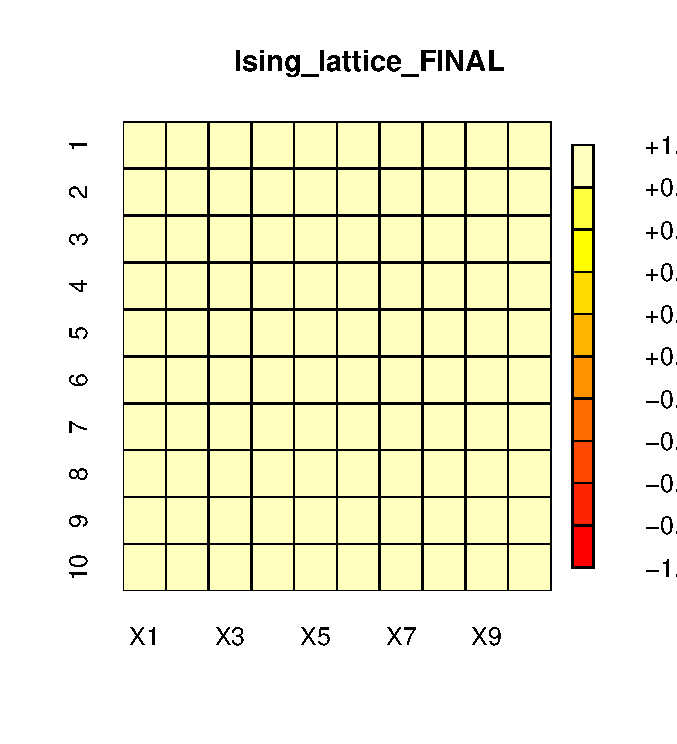
\includegraphics[width=\textwidth]{Pic/J+1_10_6000_T=0_FINAL.pdf}
     \end{center}
\end{column}
\end{columns}
\end{frame}

\begin{frame}{Ferromagnetic J=+1, T=0}
\begin{columns}
\begin{column}{0.5\textwidth}
    \begin{center}
     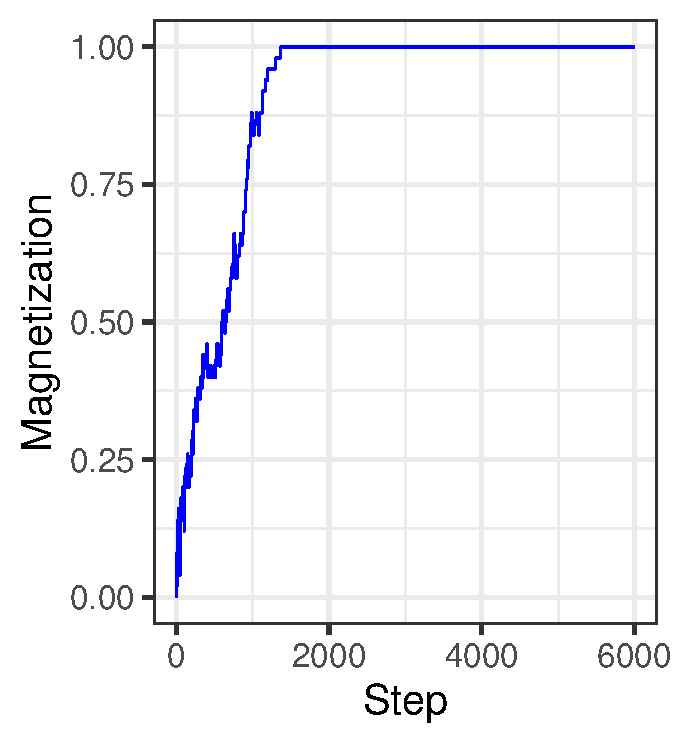
\includegraphics[width=\textwidth]{Pic/J+1_10_6000_T=0_Magnetization.pdf}
     \end{center}
\end{column}
\begin{column}{0.5\textwidth}
    \begin{center}
     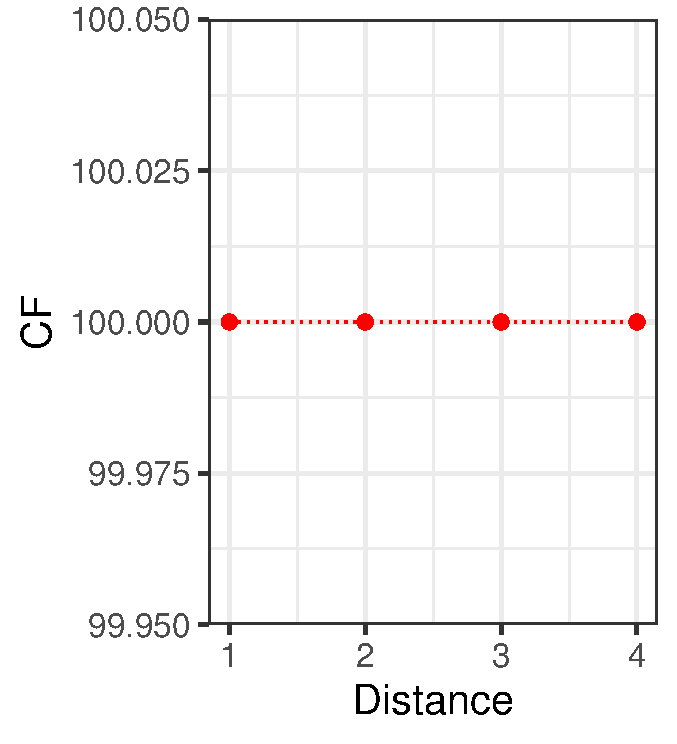
\includegraphics[width=\textwidth]{Pic/J+1_10_6000_T=0_Coherence.pdf}
     \end{center}
\end{column}
\end{columns}
\end{frame}

\begin{frame}{Ferromagnetic J=+1, T=8}
\begin{columns}
\begin{column}{0.5\textwidth}
    \begin{center}
     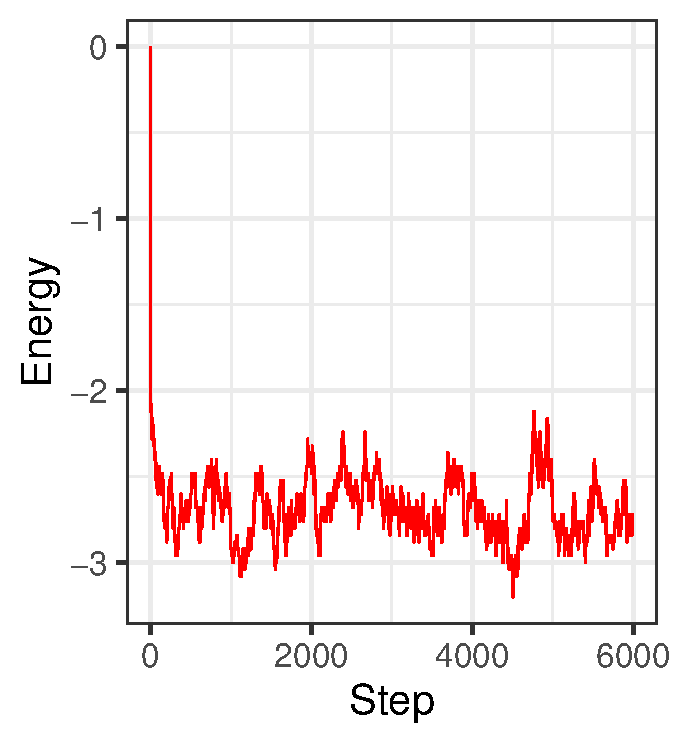
\includegraphics[width=\textwidth]{Pic/J+1_10_6000_T=8_ENERGY.pdf}
     \end{center}
\end{column}
\begin{column}{0.5\textwidth}
    \begin{center}
     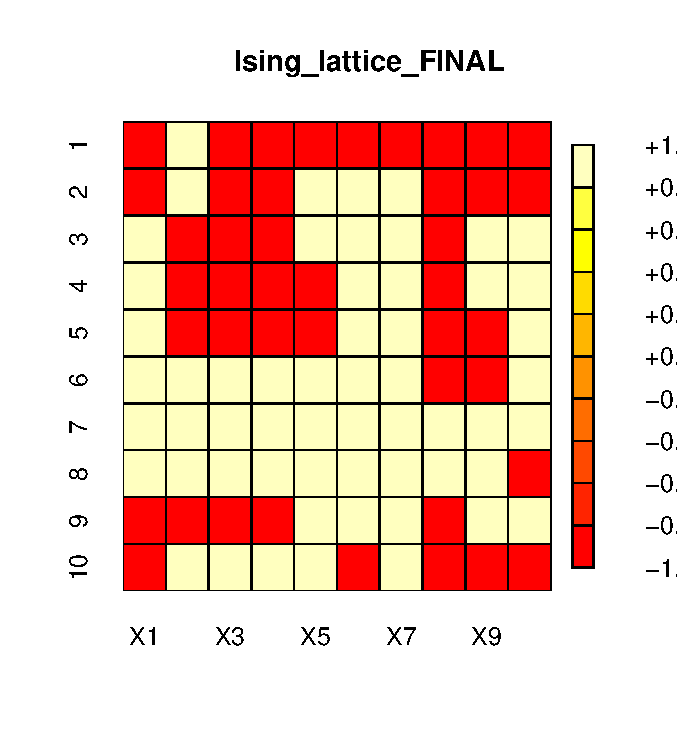
\includegraphics[width=\textwidth]{Pic/J+1_10_6000_T=8_FINAL.pdf}
     \end{center}
\end{column}
\end{columns}
\end{frame}

\begin{frame}{Ferromagnetic J=+1, T=8}
\begin{columns}
\begin{column}{0.5\textwidth}
    \begin{center}
     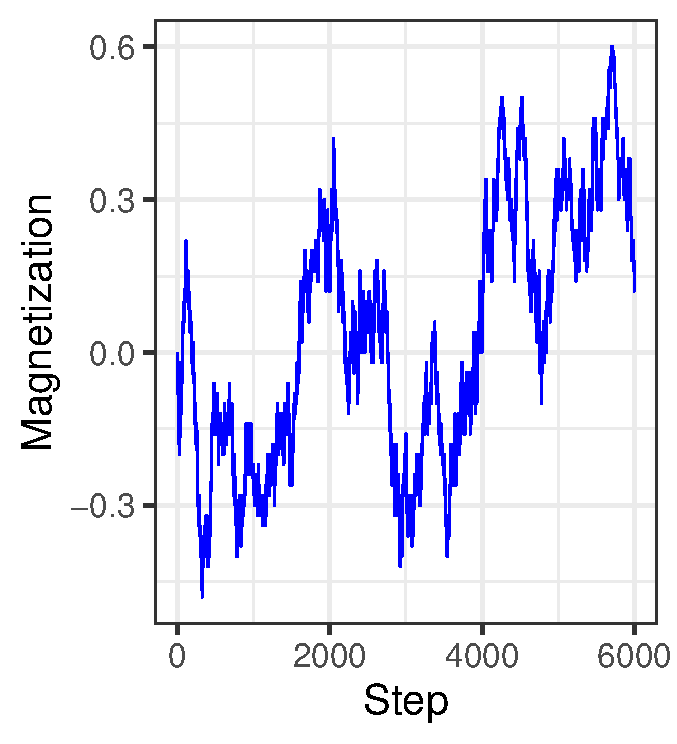
\includegraphics[width=\textwidth]{Pic/J+1_10_6000_T=8_Magnetization.pdf}
     \end{center}
\end{column}
\begin{column}{0.5\textwidth}
    \begin{center}
     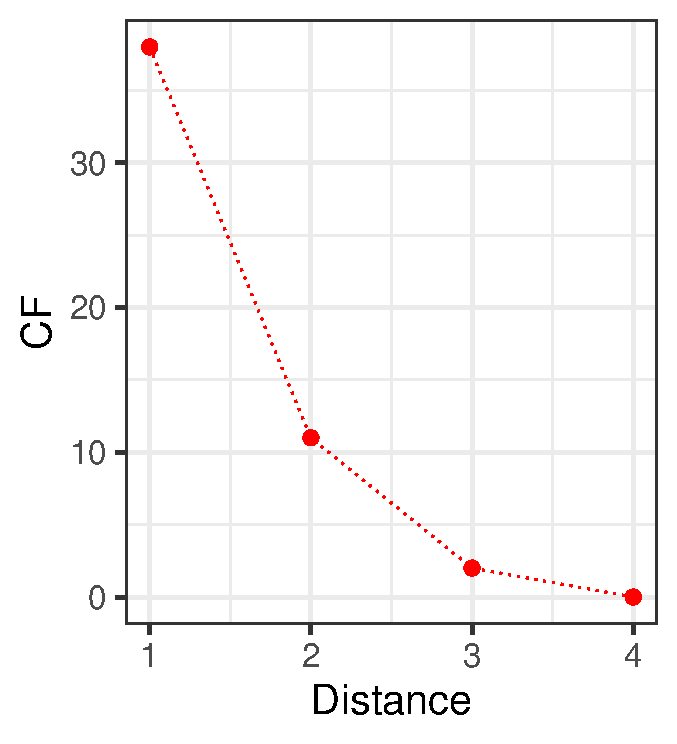
\includegraphics[width=\textwidth]{Pic/J+1_10_6000_T=8_Coherence.pdf}
     \end{center}
\end{column}
\end{columns}
\end{frame}

\begin{frame}{Ferromagnetic J=+1, T=16}
\begin{columns}
\begin{column}{0.5\textwidth}
    \begin{center}
     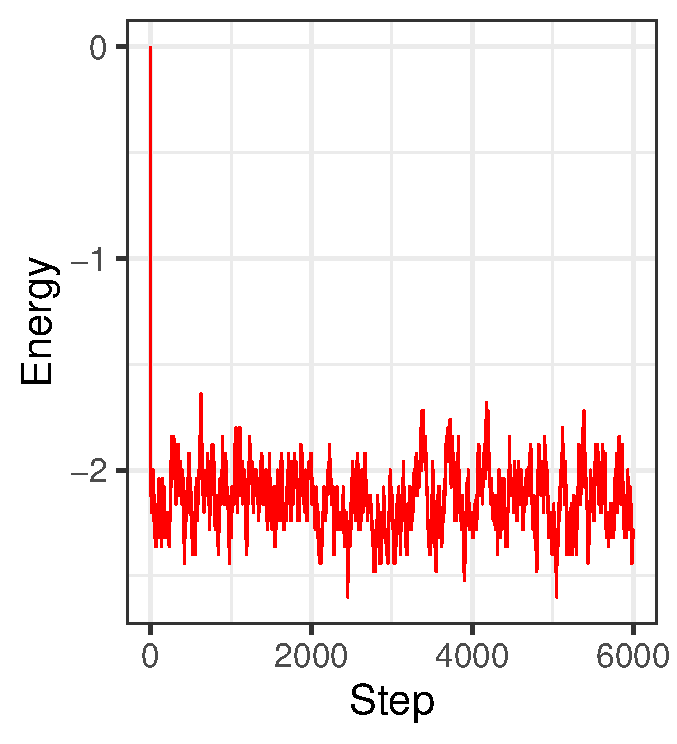
\includegraphics[width=\textwidth]{Pic/J+1_10_2500_T=16_ENERGY.pdf}
     \end{center}
\end{column}
\begin{column}{0.5\textwidth}
    \begin{center}
     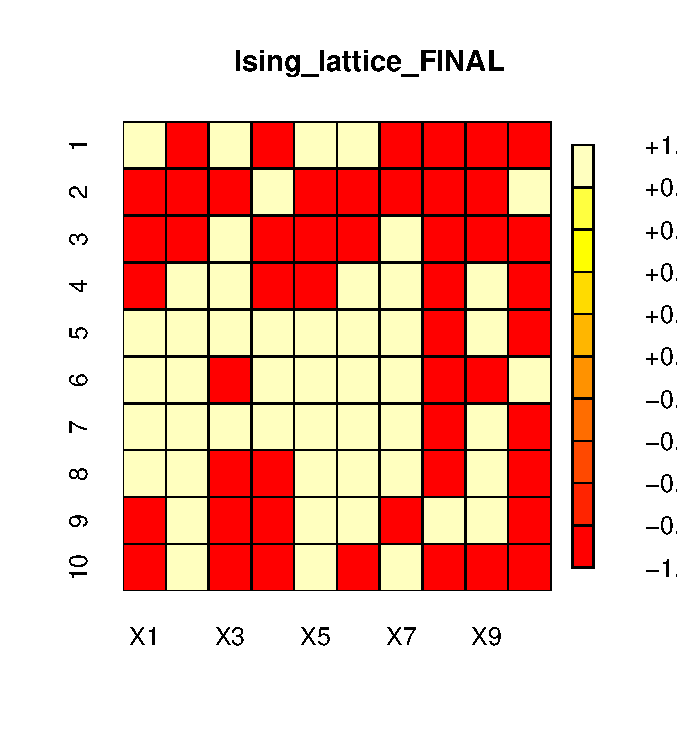
\includegraphics[width=\textwidth]{Pic/J+1_10_2500_T=16_FINAL.pdf}
     \end{center}
\end{column}
\end{columns}
\end{frame}

\begin{frame}{Ferromagnetic J=+1, T=16}
\begin{columns}
\begin{column}{0.5\textwidth}
    \begin{center}
     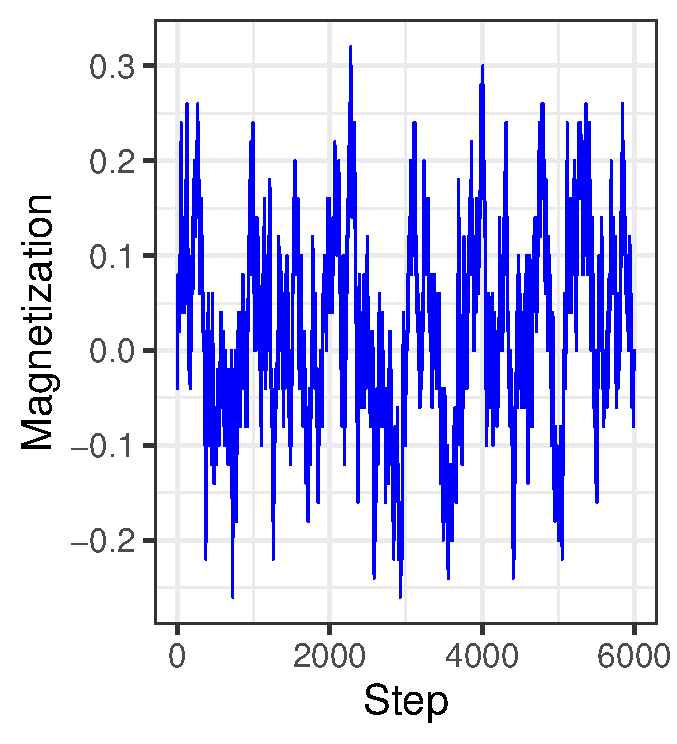
\includegraphics[width=\textwidth]{Pic/J+1_10_2500_T=16_Magnetization.pdf}
     \end{center}
\end{column}
\begin{column}{0.5\textwidth}
    \begin{center}
     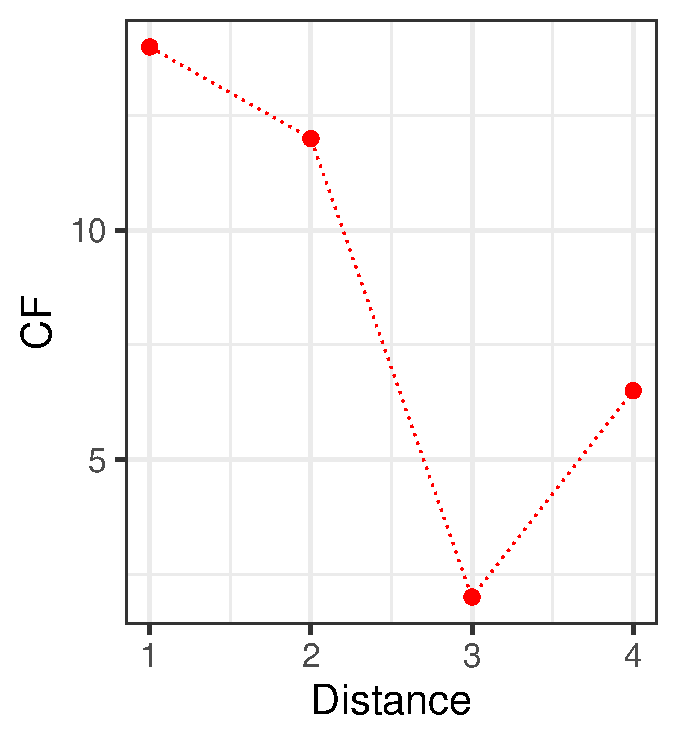
\includegraphics[width=\textwidth]{Pic/J+1_10_2500_T=16_Coherence.pdf}
     \end{center}
\end{column}
\end{columns}
\end{frame}



\begin{frame}{Ferromagnetic with two centers T=0}
    \begin{center}
     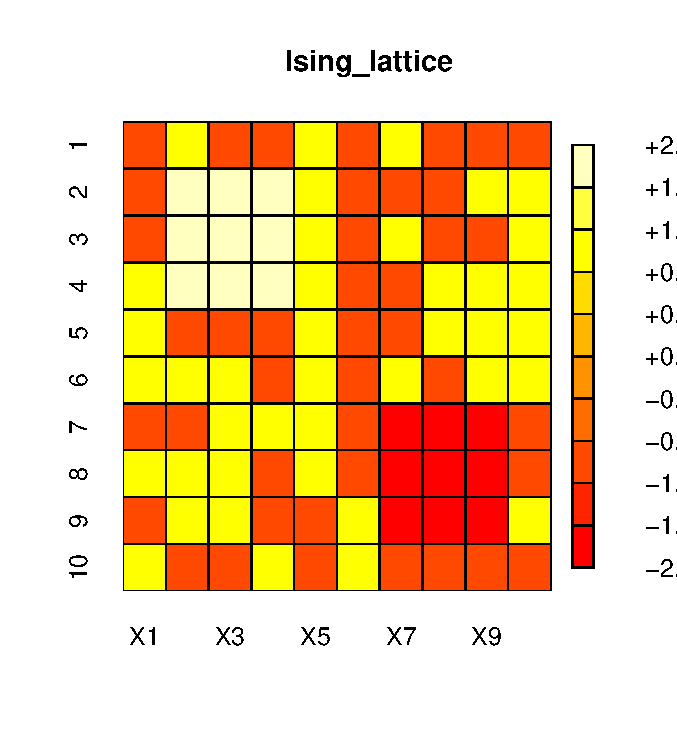
\includegraphics[width=0.5\textwidth]{Pic/2CENTER.pdf}
     \end{center}
\end{frame}


\begin{frame}{Ferromagnetic with two centers T=0}
\begin{columns}
\begin{column}{0.5\textwidth}
    \begin{center}
     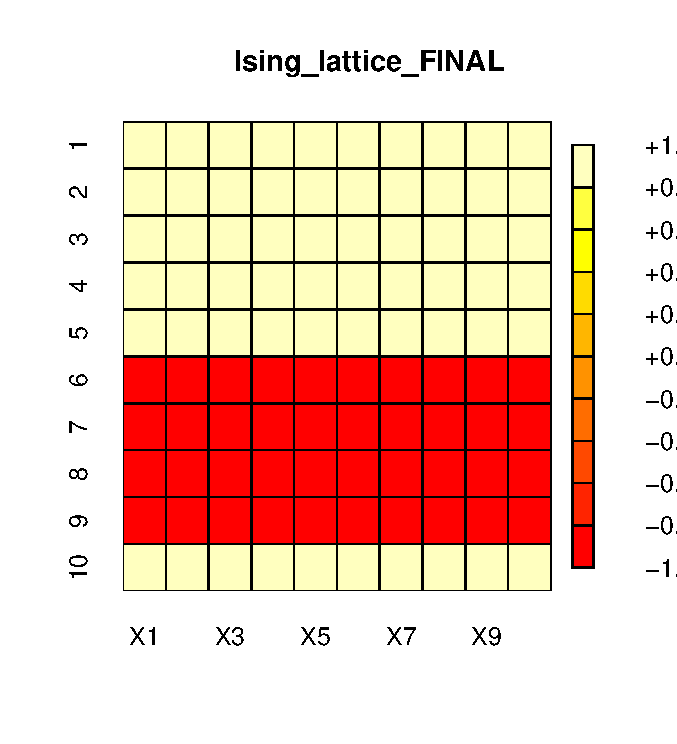
\includegraphics[width=\textwidth]{Pic/J+1_10_6000_two_center_T=0_FINAL.pdf}
     \end{center}
\end{column}
\begin{column}{0.5\textwidth}
    \begin{center}
     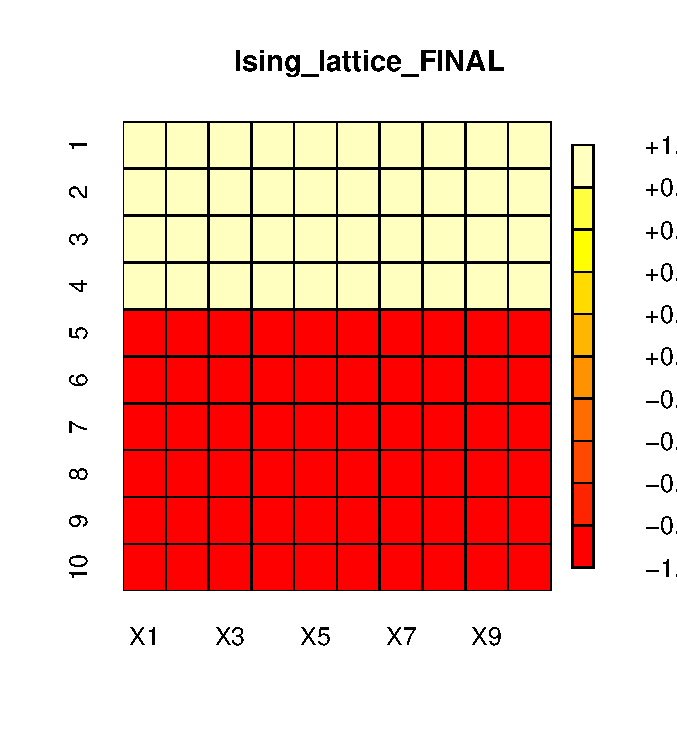
\includegraphics[width=\textwidth]{Pic/J+1_10_6000_two_center_T=0_2_FINAL.pdf}
     \end{center}
\end{column}
\end{columns}
\end{frame}


\begin{frame}{Ferromagnetic with two centers T=0, 20$\times$20}
    \begin{center}
     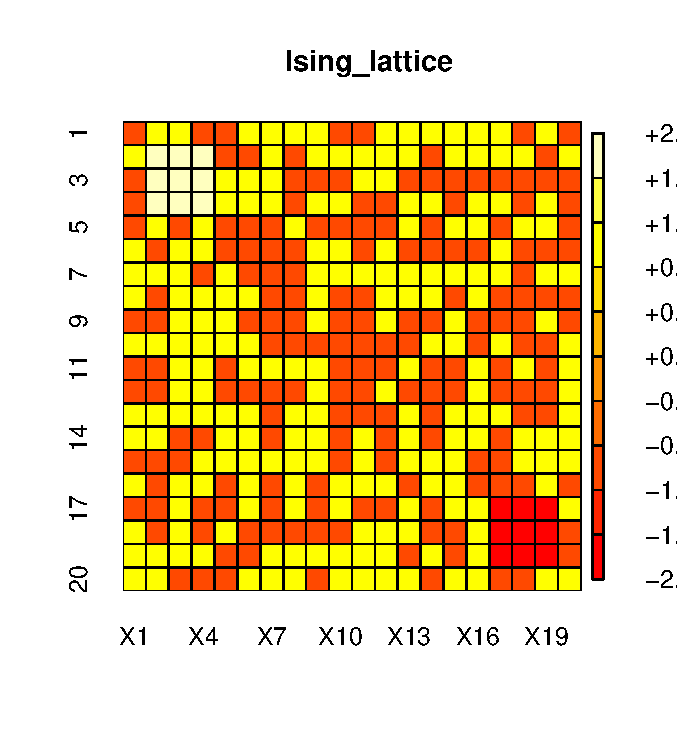
\includegraphics[width=0.5\textwidth]{Pic/LATTICE20x20TWOCENTER.pdf}
     \end{center}
\end{frame}

\begin{frame}{Ferromagnetic with two centers T=0,  20$\times$20}
\begin{columns}
\begin{column}{0.5\textwidth}
    \begin{center}
     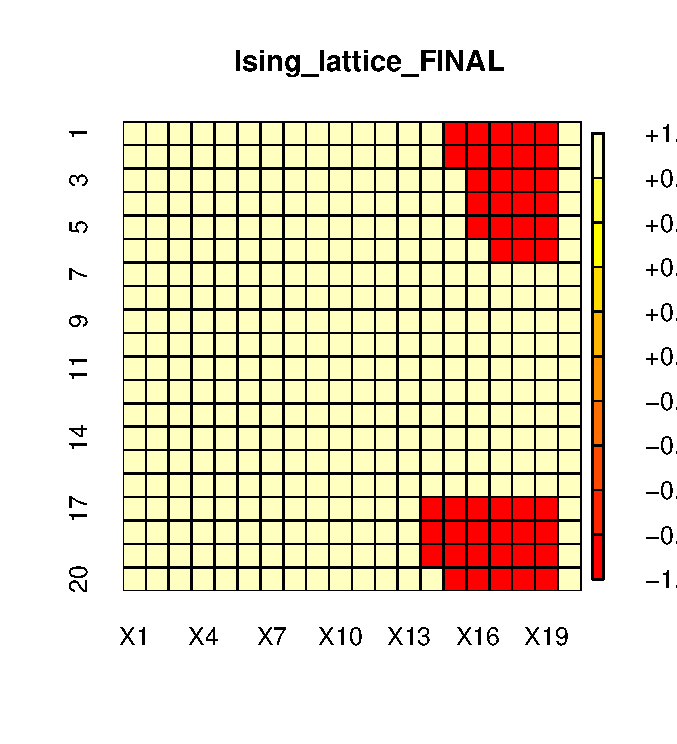
\includegraphics[width=\textwidth]{Pic/J+1_20_10000_T=0_FINAL.pdf}
     \end{center}
\end{column}
\begin{column}{0.5\textwidth}
    \begin{center}
     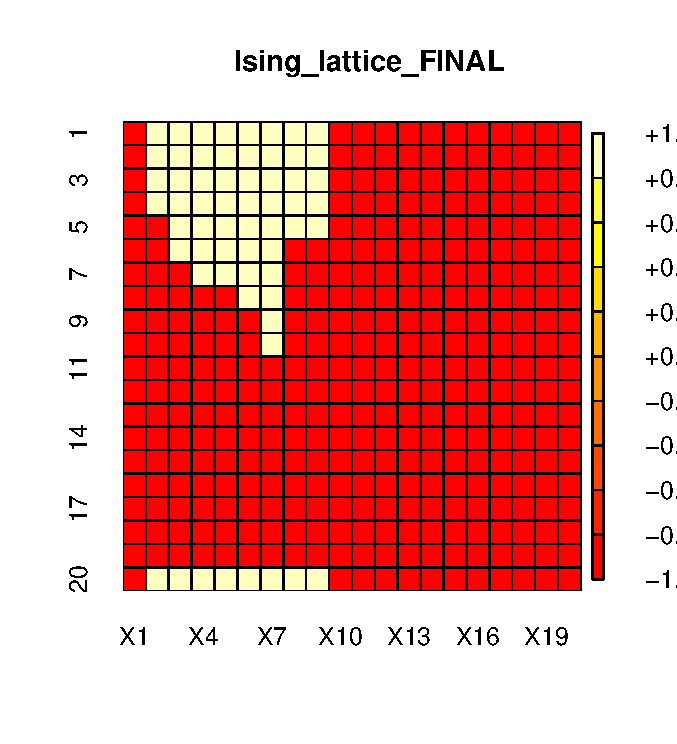
\includegraphics[width=\textwidth]{Pic/J+1_20_10000_T=0_FINAL_2.pdf}
     \end{center}
\end{column}
\end{columns}
\end{frame}







\begin{frame}[t,allowframebreaks]
\frametitle{Bibliography}
\printbibliography
\end{frame}


\section{Supporting Info}

\subsection{ROC and $\phi$ factor}
\begin{frame}{}
\begin{center}
{\Huge ROC and $\phi$ factor}
\end{center}
\end{frame}




\end{document}
